\documentclass[11pt,a4paper]{article}
\usepackage[T1]{fontenc}
\usepackage[utf8]{inputenc}
\usepackage{lmodern}
\usepackage[margin=2.5cm]{geometry}
\usepackage{booktabs,longtable,array,graphicx,url,setspace,caption,enumitem,float,pdflscape}
\usepackage[hidelinks]{hyperref}
\setstretch{1.15}
\captionsetup{font=small,labelfont=bf}
\newcommand{\todo}[1]{\textbf{[#1]}}
\makeatletter\g@addto@macro\UrlBreaks{\do\.\do\-\do\_\do\(\do\)\do\;}\makeatother
\setlength{\parskip}{0.3em}

\title{Do the gains from digital technology waves differ by income level?\\ A systematic review, a pilot meta-regression and a macro-panel analysis}
\author{Quang-Vinh Dang\thanks{British University Vietnam, Hung Yen, Vietnam. Email: vinh.dq4@buv.edu.vn. ORCID: 0000-0002-3877-8024.}}
\date{Draft of 3 October 2026}

\begin{document}
\maketitle

\begin{center}\fbox{\parbox{0.92\textwidth}{\small\textbf{Draft status (remove before submission).} All study data in this draft were extracted by machine from the full texts. Every printed number used in the meta-regression was checked against the text twice, all 77 study records were re-read once by a separate model run, a random sample of 340 screening decisions and 16 study records were redone blind by separate model runs, and the author has since checked a random sample of the extracted data by hand against the source papers \todo{author: state the sample size and the number of discrepancies}. Screening used one assisted reviewer, with an independent blind re-screening of a random sample by a separate model run. The protocol was not registered before the search was run. Scopus and Web of Science have not been searched, and Google Scholar was searched only in part (the first page of one query). Sections marked \todo{author} need the author's input. Numbers in this draft come from the files in the project repository, and the repository is the reference if text and data disagree.}}\end{center}

\begin{abstract}
\noindent\textbf{Background.} Mobile telephony, the internet and, more recently, artificial intelligence (AI) are often expected to widen or narrow income gaps between countries, but the empirical cross-country evidence has not been synthesised across outcomes. \textbf{Methods.} We ran a systematic review following PRISMA 2020, searching OpenAlex, Crossref and NBER for 1995 to 2026 and, as a supplement, one page of a Google Scholar query, and assessed 118 full texts. We extracted effects on six outcome families, rated risk of bias with an adapted ROBINS-I tool, synthesised results narratively, and ran a pilot meta-regression of partial correlations for ICT-type adoption and output or productivity. For questions the studies cannot answer, we analysed World Bank data for 1995 to 2019 with fixed-effects panels, a staggered event study with not-yet-treated controls and local projections. \textbf{Results.} Seventy-seven studies met the criteria (62 on ICT, mobile, internet and broadband; 13 on AI; 2 on both). None was rated at low risk of bias (moderate 9, serious 59, critical 9). Most studies report a positive association between ICT-type adoption and output, but the pooled partial correlation across 18 studies is 0.17 (95\% CI 0.09 to 0.25) with I$^2$ of 93\%, and falls to between 0.06 and 0.09 after correcting for small-study bias. The moderator results are not stable: GMM estimates were 0.16 lower than others in a first run, and 0.16 higher once two studies found later were added, and restricting to studies with an identification strategy raises the pooled value instead of lowering it. Thirty-three studies compare income groups or regions: eight find larger effects in richer economies, nine in poorer ones, and four find no difference, mostly without a formal test. Returns are conditional on human capital, financial depth, governance and infrastructure. Evidence on AI comes from 15 studies, mostly short and using proxies. In the World Bank panel, mobile adoption was associated with faster growth in every income group under a same-period specification, most strongly in lower-middle income economies, but no income group showed a positive association under all four designs (same-period and predetermined panels, a staggered event study and local projections). \textbf{Conclusions.} The evidence does not establish that rich or poor economies gain more, and it cannot support causal statements. Credible identification for low- and middle-income economies is the main gap.
\par\medskip\noindent\textbf{Keywords:} digital technology; ICT; artificial intelligence; income level; systematic review; meta-regression; event study.\\
\textbf{JEL codes:} O33, O47, O11, L96.
\end{abstract}

\newpage

\section{Introduction}

Whether new technologies narrow or widen income gaps between countries is a long-standing question, and it has returned with artificial intelligence. Early empirical work found sizeable output effects of telecommunications infrastructure \cite{roller2001}. Later work on the long-run diffusion of technologies finds that technologies arrive at similar times in rich and poor countries, but that the intensity of their use diverges \cite{comin2010,comin2018}. If so, the gains from a new technology should depend on a country's conditions at the time of adoption, and not only on whether the technology has arrived.

Evidence on this is scattered. Studies use different technologies (mobile subscriptions, internet users, composite ICT indices, ICT capital, robots, AI readiness indices), different outcomes (growth, productivity, employment, inequality, human development, emissions), different samples and different estimators. Individual studies often report one average effect and one or two interaction terms. A reader who wants to know whether a low-income economy can expect the same payoff as a high-income one has no single place to look, and a policymaker who reads one study can reach the opposite conclusion from one who reads another.

We therefore ask the following main question: \emph{in empirical cross-country studies of digital and general-purpose technology waves, do the effects on output, structural change, labour markets, distribution, living standards and resource use differ by income level and by country characteristics, how large are the differences, and how credible is the evidence?} We keep studies of historical waves (ICT, mobile, internet, broadband, crypto-assets) separate from studies of AI, because AI evidence is younger and thinner. We also ask a set of subsidiary questions that the data we collected allow, and four questions that the published studies cannot answer, which we address with World Bank data.

The paper has three parts. The first is a systematic review that follows PRISMA 2020, with a structured extraction of effects, a quality rating of each study and a narrative synthesis across six outcome families. The second is a pilot meta-regression of effect sizes for the best-covered question, the association between ICT-type adoption and output or productivity, together with nine exploratory questions about measurement, study design and the conditions under which returns differ. The third is an original analysis of World Bank panel data that gives a first, transparent answer to four questions about the shape of the effect by adoption level, effects by income group under one design, timing around technology arrival, and differences inside low-income economies.

The contribution is a map of the evidence with an explicit quality rating of each study, a transparent count of where income-group comparisons exist and where they do not, an estimate of how much of the apparent positive association survives bias corrections, and a panel analysis whose limits are stated at each step. We are explicit about what the data cannot show. All data and code are in the project repository.

The rest of the paper is organised as follows. Section~\ref{sec:background} sets out the conceptual background and the hypotheses. Section~\ref{sec:methods} describes the methods. Section~\ref{sec:results} reports the review and the meta-regression, and Section~\ref{sec:panel} reports the panel analysis. Section~\ref{sec:discussion} discusses the findings, and Sections~\ref{sec:limits} and~\ref{sec:conclusion} give the limitations and conclusions.

\section{Conceptual background and hypotheses}\label{sec:background}

\subsection{Why the same technology could pay differently}
Four mechanisms recur in the literature on information and communication technology and on automation, and each implies a reason why the gain from a technology might differ by income level.

\emph{Infrastructure and complementary investment.} Telecommunications infrastructure raises output, and the effect may depend on how much infrastructure already exists, because network benefits grow with the size of the network \cite{roller2001}. Where electricity, roads and financial services are scarce, the same handset or connection may yield less. This implies that the gain depends on a country's stock of complementary assets, which is usually lower in poorer economies.

\emph{Information and market access.} Mobile phones can reduce price dispersion and waste where markets are thin. In a study of South Indian fisheries, the arrival of mobile phones reduced price dispersion and waste and raised welfare \cite{jensen2007}, and a review of evidence from Africa describes how mobile phones can improve information flows in agricultural and other markets \cite{aker2010}. These mechanisms are strongest where information was previously scarce, which is more common in lower-income settings, and they imply large early gains at low adoption levels.

\emph{Skills and tasks.} Computers substitute for routine tasks and complement non-routine tasks \cite{autor2003}, and automation both displaces and creates tasks \cite{acemoglu2019}. In Africa, the arrival of fast internet through submarine cables was associated with higher employment, and the effect was larger for more skilled workers \cite{hjort2019}. The gains therefore depend on the skills of the workforce, which differ by income level.

\emph{Absorptive capacity.} The ability to use external knowledge depends on prior related knowledge \cite{cohen1990}. For technology adoption this means that returns depend on human capital, management capacity and institutions, again variables that differ systematically by income.

Two forces therefore pull in different directions. Catch-up and early information gains suggest that low-adoption, lower-income economies could gain more per unit of adoption. Complementary assets, skills and absorptive capacity suggest that higher-income economies could gain more. A third consideration is time: the long-run diffusion evidence suggests that gains may build over years, and a short window may miss them \cite{comin2018}. A review of the empirical evidence on information technology and economic performance, published early in the period we study, describes the findings as mixed \cite{dedrick2003}; it is not an estimating study and is not among our included studies.

\subsection{Hypotheses and questions}
These mechanisms lead to the following hypotheses, which structure the review and the panel analysis. They are stated so that the data can contradict them.

\begin{description}[leftmargin=1.4em,itemsep=2pt]
\item[H1] ICT-type adoption is positively associated with output and productivity, but the size of the association is modest and varies strongly across studies.
\item[H2] The association is larger where complements are stronger: higher human capital, deeper financial markets, better governance and better infrastructure.
\item[H3] The association differs by income level, but its sign is not predicted, because catch-up and complement effects have opposite implications.
\item[H4] Estimates from designs that address reverse causation are smaller than those from designs that do not.
\item[H5] Gains depend on timing, appearing with a lag, so that studies measuring only contemporaneous effects understate them.
\item[H6] Evidence on AI follows the same pattern as evidence on earlier technologies but is thinner and of lower quality.
\end{description}

\section{Methods}\label{sec:methods}

\subsection{Protocol and registration}
The review follows PRISMA 2020 \cite{prisma2020} and the structure of PRISMA-P \cite{prismap}. The protocol (version 1.0, 2 October 2026) is in the repository. It was intended to be registered on the Open Science Framework before the search, but registration had not been completed when the search was run. This is a deviation from good practice, and we log the amendments made after the search in Appendix~\ref{app:amend}. \todo{author: register the protocol on OSF and state the registration number or explain}

\subsection{Eligibility criteria}
We included quantitative empirical studies with their own estimation (panel regression, instrumental variables, growth accounting, event studies, structural estimation) that relate adoption, diffusion, investment or capability of ICT in general, mobile telephony, internet or broadband, crypto-assets or AI to at least one outcome in six families: (1) output and productivity, (2) structural change, (3) labour market, (4) poverty and distribution, (5) living standards beyond income (consumption, health, schooling, financial inclusion) and (6) resource cost (electricity use, carbon intensity). Historical-wave studies needed at least 10 economies or an explicit income-group comparison; AI studies needed at least 3 economies or an income-level comparison. Studies from 1995 onward in English were eligible. Purely conceptual papers, reviews and studies whose only outcome was adoption itself were not synthesised. Full criteria and exclusion codes are in Appendix~\ref{app:criteria}.

\subsection{Information sources and search}
We searched OpenAlex (a Boolean query restricted to the economics field), Crossref (96 technology-by-context queries) and the NBER working-paper series, covering 1995 to the search date of 2 October 2026. The search blocks and the OpenAlex query are in Appendix~\ref{app:search}. arXiv was attempted but did not respond in usable time. Scopus, Web of Science and EconLit were not searched, because they need institutional access. After removing duplicates by DOI and by normalised title and year, 3,612 records remained.

A blind re-screening of the retrieved records suggested that the search had missed relevant studies (Section~\ref{sec:crosscheck}). A first supplementary check in Google Scholar, where the author ran one query (G1, listed in the repository) and passed on its first page of 10 results, found that 9 of the 10 were not among the 3,612 records. Those nine are handled outside the main flow (Table~\ref{tab:prisma}); the other 14 planned Google Scholar queries have not been run, and the search as a whole should therefore be regarded as incomplete.

\subsection{Screening and full-text access}
Screening was done by one assisted reviewer. Automated rules removed records with no eligible technology term, no outcome term or no multi-economy cue (stage 1). Title and abstract screening then applied the eligibility table, with four holding categories for records that were not eligible but useful (context on diffusion, environmental-only outcomes, reviews for citation search and supplementary micro evidence). No human second screener was available. Instead, a separate model run, which saw only the criteria and each record's title and abstract, independently re-screened a random sample of 340 records (100 of those removed by the automated rules, 120 of those removed at title level and 120 of those assessed at abstract level; seed 20261004). Records the first screener excluded and the second would include were adjudicated by a third blind reading of the abstract. We report agreement and an estimate of missed records in the Results. A further 90-decision sample for a human check is in the repository.

Full texts were obtained from open-access sources, repositories and the author. Records without a free full text, and those the author judged to come from unreliable venues after visiting the journal site, were not read and are not used as evidence. This creates a selection mechanism that favours open-access studies; Section~\ref{sec:limits} discusses it. Three studies were added late (71, 278 and 341) after the author supplied them; one further study (89) was supplied and excluded. After the blind re-screening, five more records it flagged were obtained and read: four are included (448, 755, 891 and 9001) and one (474) was excluded. The six studies from the Google Scholar page that the author could download (9101 to 9106) were read, extracted and checked in the same way as the others; three further results of that page (Chavula 2013, Torero et al. 2006 and a 2026 preprint) could not be obtained.

\subsection{Data extraction}
For each included study we extracted technology, exposure measure, sample, estimator, identification strategy, results by outcome family with printed estimates and uncertainty, heterogeneity findings, and group-specific results, using a fixed form (Appendix~\ref{app:criteria}). Extraction was done by a language-model agent working from converted full texts, with a locator and a short verbatim quote for every result. An automatic check matched 477 of 694 quotes verbatim across all 118 records read (the remainder are affected by table layout and paraphrase).

\subsection{Second-pass check}
A second, separate model run then re-read each of the 77 included records and each of 251 regression estimates against the text and classified every item as confirmed, corrected or unverifiable. This catches transcription and reading errors. It is not an independent check: the same family of model reads the same machine-converted text, and garbled tables stay garbled. Appendix~\ref{app:secondpass} summarises the second pass by study. In addition, a separate model run independently re-extracted key fields (number of economies, years, estimator class, identification, outcome families, headline direction on output, income-group comparison, low-income coverage and overall risk of bias) for 16 randomly chosen included studies (drawn before the six Google Scholar studies were added) without seeing the original extraction, and we compare the two. Finally, the author checked a randomly selected sample of the extracted data by hand against the source papers. \todo{author: number of studies and entries in the sample, number of discrepancies and how they were resolved}

\subsection{Risk of bias}
Risk of bias used a six-domain tool adapted from ROBINS-I \cite{robinsi}: confounding and reverse causation, exposure measurement, selection of countries and years, outcome measurement, specification and researcher degrees of freedom, and selective reporting. The overall rating was low, moderate, serious or critical, with the definitions in Appendix~\ref{app:criteria}. One rater made the first-pass ratings; the second pass offered an opinion on each, which we report without changing the ratings.

\subsection{Narrative synthesis}
We synthesised results narratively, following the SWiM reporting guideline \cite{swim}, by outcome family and by technology stream. Studies were grouped by outcome family; within each family we tabulated the direction of the results, the estimator, the sample and the risk of bias (Appendix~\ref{app:families}). Counts of study directions are descriptive; they are not weighted by sample size or quality and are not effect sizes.

\subsection{Pilot meta-regression}
For ICT-type adoption and output or productivity we ran a pilot meta-regression in the tradition of Stanley and Doucouliagos \cite{stanley2012}. Each estimate was converted to a partial correlation coefficient, $PCC = t/\sqrt{t^2 + df}$, with standard error $\sqrt{(1-PCC^2)/df}$ and $df$ equal to the number of observations minus 10 regressors (a sensitivity check uses 0, 5 and 20). The $t$-statistic came from the printed coefficient and standard error, or from a printed $t$-statistic. Estimates reported with $p$-values or intervals only were not converted. We excluded interaction terms, crypto and AI exposures, estimates without a usable number of observations, and five estimates judged not poolable on the second pass (a fintech-credit exposure, a growth outcome mixed with level outcomes, and a TFP index in levels). We pooled one headline estimate per paper by random effects \cite{dersimonian1986}, ran a weighted moderator regression with standard errors clustered by paper, and tested for publication selection with the funnel-asymmetry and precision-effect tests (FAT-PET) and the precision-effect estimate with standard error (PEESE) \cite{stanley2014}. With 20 papers, the clustered standard errors are optimistic and p-values are indicative.

\subsection{Additional exploratory questions}
Beyond the main question we specified nine further questions and their analyses before running them (\texttt{review/extra\_questions\_spec.md}), all using the data already collected: whether the pooled association depends on the measurement of the technology (a composite index versus a single indicator), on the outcome form (growth versus level) and on the sample period (added one at a time to the meta-regression); whether weaker designs are more common where low-income economies are sampled; whether study quality goes with the reported direction; which enabling conditions authors test and in which direction (153 heterogeneity entries classified by one model reader, with a second reader on a random 20\% sample); the thresholds stated; an evidence-gap map by outcome family and income group; and a comparison of the AI and historical-wave streams. These analyses are exploratory, are not corrected for multiple testing, and should be read as hypotheses.

\subsection{Macro-panel analysis}
Four questions (the shape of the effect by adoption level, effects by income group under one design, timing around technology arrival, and differences inside low-income economies) cannot be answered from the included studies. We therefore specified, before downloading the data, an analysis of public World Bank World Development Indicators for 1995 to 2019 (\texttt{analysis/spec.md}), and later amended the event-study design (\texttt{analysis/spec\_amendment.md}) after the first design failed its own checks. The variables and their World Bank codes are in Appendix~\ref{app:panel}.

\emph{Fixed-effects panels (A1 to A3, A6).} In five-year periods (1995--2000, 2000--05, 2005--10, 2010--15 and 2015--19), annual growth of GDP per capita was regressed on the change in mobile subscriptions per 100 people over the same period (A1) or the previous period (A2), with initial log income, initial gross secondary enrolment, the change in trade openness and period effects, separately by current World Bank income group, with standard errors clustered by country. A3 splits the change by baseline adoption level, and A6 adds enabling conditions inside low and lower-middle income economies, one moderator at a time.

\emph{Event study (A4b).} The takeoff year is the first year mobile subscriptions reach 10 per 100 people among economies below that level in 1995. For each cohort of economies with the same takeoff year and each horizon from five years before to ten years after, the effect compares the change in log GDP per capita from the year before takeoff with the change in economies not yet treated at that horizon, after adjusting for initial income and earlier growth by outcome regression, in the manner of Callaway and Sant'Anna \cite{callaway2021}. Estimates are averaged across cohorts, weighted by the number of treated economies, and intervals come from a bootstrap over economies. Effects at horizons before takeoff are placebo tests, and a subgroup is interpreted only if the interval of their mean includes zero. We use not-yet-treated controls because standard two-way fixed-effects event studies can be biased when treatment is staggered and effects vary over time \cite{sun2021,dechaisemartin2020}.

\emph{Local projections (A7).} For a design without a binary treatment, we estimated local projections \cite{jorda2005} on the annual panel: cumulative growth of GDP per capita from year $t$ to $t+h$ on the change in mobile subscriptions over the previous three years, with country and year fixed effects, controls for earlier growth and initial income, and separate coefficients by income group.

All of these are associations. We have no instrument, so we do not claim a causal effect, and cost-effectiveness cannot be examined with these data.

\section{Results of the review and the meta-regression}\label{sec:results}

\subsection{Study selection}
Figure~\ref{fig:prisma} and Table~\ref{tab:prisma} give the flow. Of 247 records sent to full-text assessment, 106 full texts were obtained and read, together with one review, five records outside the 247 that the blind re-screening flagged (Section~\ref{sec:crosscheck}) and six records found through Google Scholar. After the second pass, 77 studies are included, 40 were excluded at full text (13 for too few economies, 5 for an ineligible exposure, 1 for an ineligible outcome, 21 for being conceptual or lacking their own estimation) and one was kept as context. Four studies (298, 474, 878 and 1495) were moved from include to exclude after the second pass on eligibility grounds; this should be confirmed by a human reviewer. About 140 of the 247 records have not been read because no free full text was available.

\begin{figure}[ht]\centering
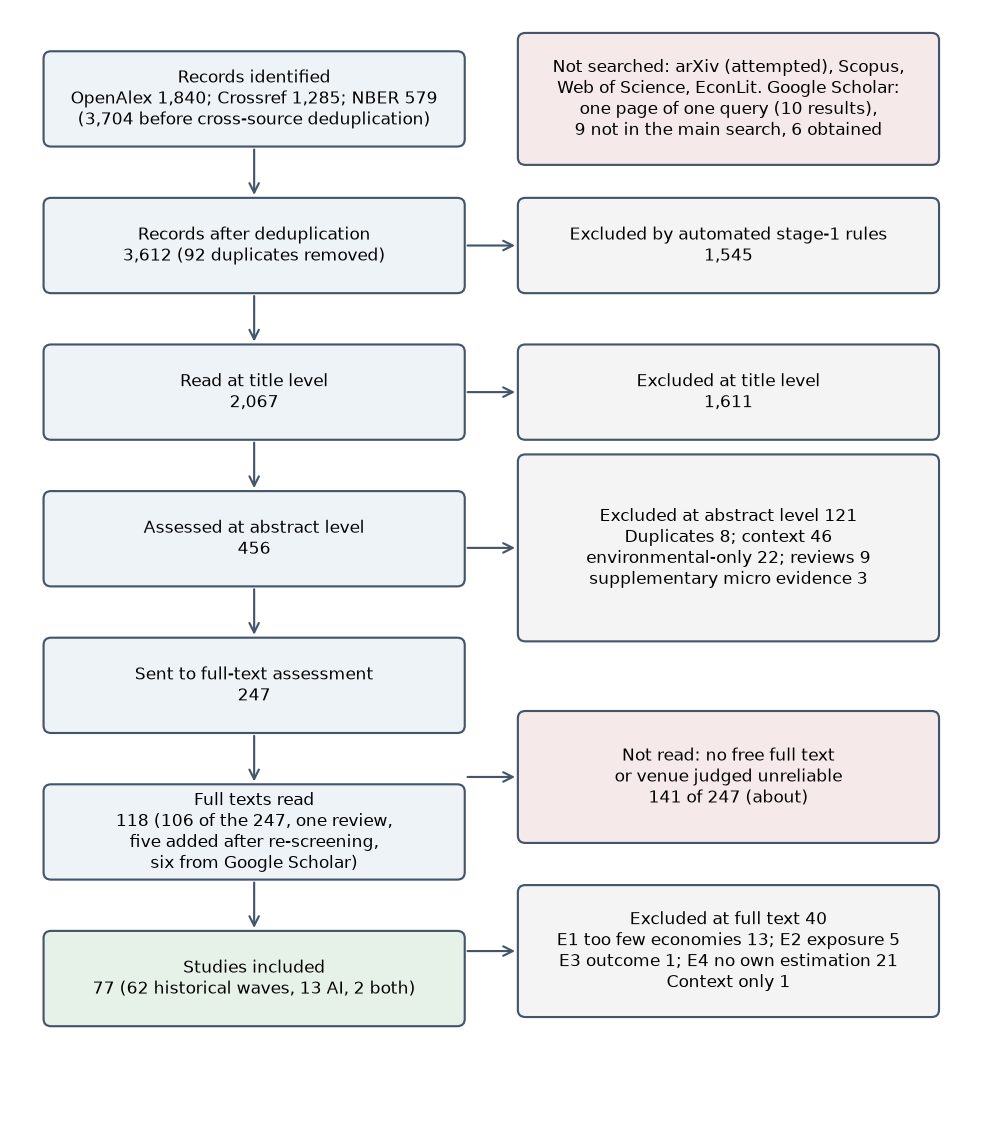
\includegraphics[width=0.78\textwidth]{fig_prisma.png}
\caption{PRISMA 2020 flow diagram.}\label{fig:prisma}
\end{figure}

\begin{table}[ht]\centering\small
\caption{Study selection (counts from the project repository).}\label{tab:prisma}
\begin{tabular}{@{}p{12.2cm}r@{}}\toprule
Stage & n\\\midrule
Records identified (OpenAlex 1,840; Crossref 1,285; NBER 579; before cross-source deduplication 3,704) & 3,704\\
Duplicates removed across sources & 92\\
Records after deduplication & 3,612\\
Google Scholar, query G1 page 1 (supplementary): results / not in the main search / obtained and read & 10 / 9 / 6\\
Excluded by automated stage-1 rules & 1,545\\
Read at title level / excluded at title level & 2,067 / 1,611\\
Assessed at abstract level / excluded at abstract level & 456 / 121\\
Held as duplicates, context, environmental-only, reviews, supplementary & 88\\
Sent to full-text assessment & 247\\
Full texts read (106 of the 247, one review, five records added after the re-screening and six from Google Scholar) & 118\\
Excluded at full text & 40\\
Kept as context only & 1\\
\textbf{Included} & \textbf{77}\\\bottomrule
\end{tabular}\end{table}

\subsection{Characteristics of included studies}
The 77 included studies were published between 2003 and 2026, and 61 of them from 2020 onward (Figure~\ref{fig:years}). Sixty-two study ICT, mobile, internet or broadband; 13 study AI; 2 cover both. Most use country-year panels (61), with a few at industry-country level. In a rough classification of the main estimator, 28 use system or difference GMM, 29 use fixed-effects, random-effects or pooled OLS, 12 use ARDL, cointegration or heterogeneous-panel estimators and 8 use growth accounting, data envelopment or other methods. Thirty-nine studies have no identification strategy beyond controls and fixed effects. Twenty-four list at least one low-income economy; studies that do not state their income coverage are counted as not listing one. Outcome families, with a study able to contribute to several, are: output and productivity 44, labour market 14, living standards beyond income 15, poverty and distribution 11, structural change 6, resource cost 6. Appendix~\ref{app:studies} lists all studies and Appendix~\ref{app:families} gives the results by family.

\begin{figure}[ht]\centering
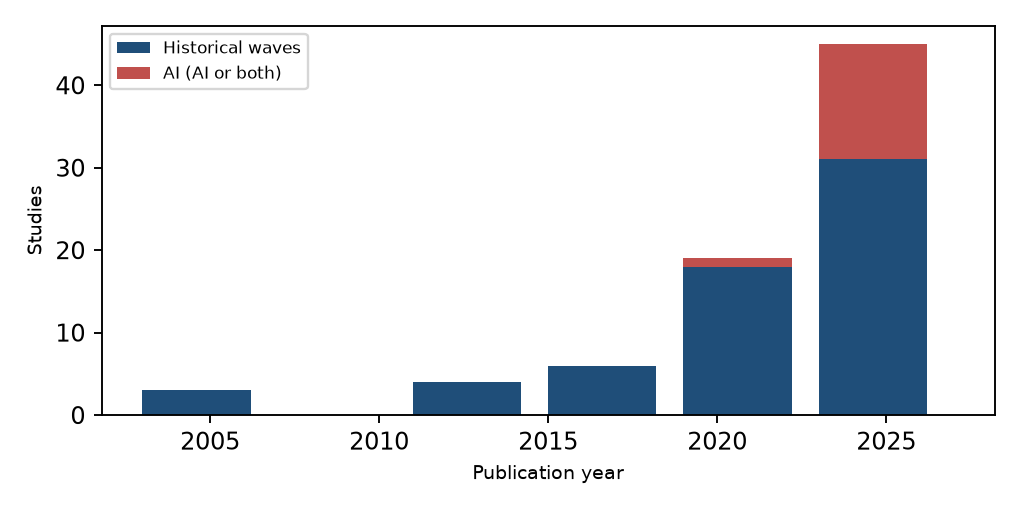
\includegraphics[width=0.62\textwidth]{fig_years.png}
\caption{Included studies by publication year and stream.}\label{fig:years}
\end{figure}

\subsection{Risk of bias}
No study was rated at low risk of bias. The first-pass ratings were moderate for 9 studies, serious for 59 and critical for 9 (Figure~\ref{fig:rob}). In the second pass, the separate reader agreed with the overall rating for 68 of 77 studies, found six too harsh (268, 302, 323, 408, 707 and 1469) and three too lenient (57, 957 and 1031). We did not change any rating, and these differences should be settled by a human reviewer. The commonest weaknesses are adoption treated as exogenous, indices whose scope does not match the technology, and many specifications with no stated preferred one.

\begin{figure}[ht]\centering
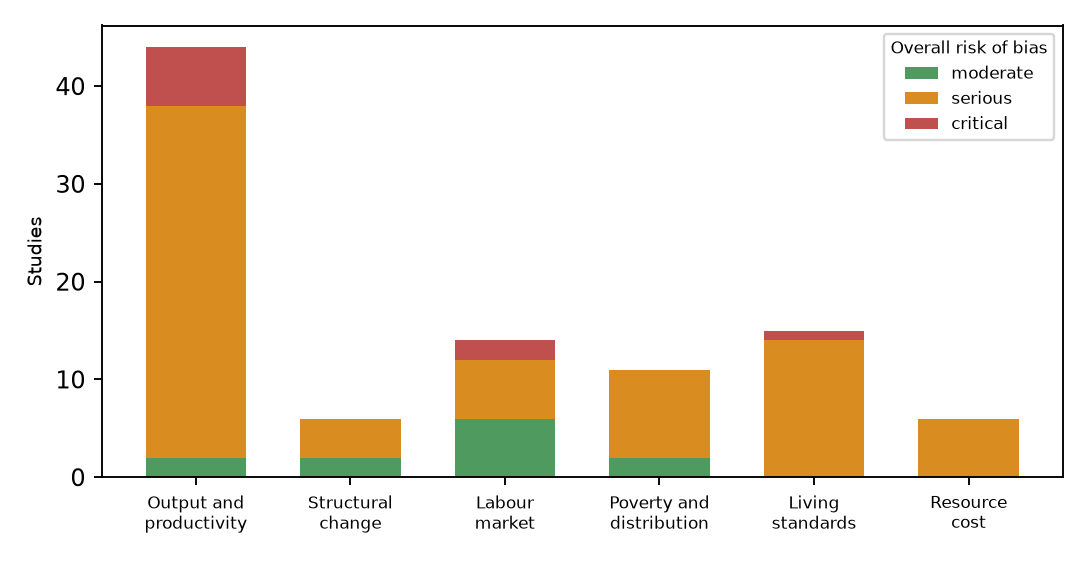
\includegraphics[width=0.66\textwidth]{fig_rob.png}
\caption{Overall risk of bias by outcome family (a study counts in each family it reports).}\label{fig:rob}
\end{figure}

\subsection{Accuracy of the extraction}
Across 461 result entries in the 77 re-read records, 425 were confirmed, 31 corrected and 5 could not be verified; 16 of 153 heterogeneity entries were corrected. Of 251 regression estimates, 245 matched the printed tables and six needed correction: one income label and the five estimates of study 9103, which had been read from the wrong cell of a panel-VAR table (rows are equations and columns lagged regressors, as the paper's own Granger tests show, whereas its text reads the table the other way). In that study the extraction had followed the paper's text, so the second pass caught an error that originated in the source and that the first pass had copied. Corrections were mostly misread labels, counts, and claims that the source text does not make. They were applied or flagged in the repository. Because both passes used the same family of model reading the same machine-converted text, the author's hand check against the source papers is therefore the reference. \todo{author: report agreement and corrections}

\subsection{Independent cross-checks of screening and extraction}\label{sec:crosscheck}
\emph{Screening.} The blind second screener agreed with the first on whether to send a record to full text for 79\% of the 120 records in the abstract-stage sample (Cohen's kappa 0.59 when its ``unsure'' counts as include and 0.54 when it does not). Its disagreements were mostly cases where it was more inclusive: of the 72 records the first screener did not send forward, it would have included or flagged 20. Of the 8 sampled records the first screener set aside as environmental-outcome-only (protocol amendment 2), the second screener would have sent 7 to full text. Carbon and electricity outcomes are in outcome family 6, so such records meet the eligibility criteria; setting them aside was a prioritisation choice, and it explains in part why only four included studies report resource-cost outcomes.

\emph{Recall.} Among the records excluded earlier, the second screener would have included or flagged 7 of 100 (automated rules), 15 of 120 (title level) and 8 of 120 (abstract level, coded exclusions). After a third blind reading of the abstracts, 2 of 100, 10 of 120 and 4 of 120 met or probably met the criteria. Extrapolated, this implies roughly 31 (range 9 to 108), 134 (74 to 236) and 15 (6 to 38) missed records at the three stages, on the order of 180 in total (range about 90 to 380). These are small samples read by model readers, and 9 of the 30 adjudicated records had no abstract, so the figure is a warning about recall and not a count. A later first-page check of one Google Scholar query found 9 of 10 results missing from the 3,612 records, and six of them were included, so the main search had poor recall for this question and the estimate above is a lower bound. The missed records are typically AI or digital-economy panels with carbon or energy outcomes, small AI panels, and financial-inclusion studies in Africa and the Arab world. Adding two such studies reversed the sign of some moderator estimates in the meta-regression (Section~\ref{sec:results}), so conclusions that rest on moderators are fragile, and the evidence base is smaller than the literature.

\emph{Extraction.} A blind re-extraction of key fields for 16 random included studies agreed with the original on the outcome families (16 of 16), start and end year (15 of 16 each), the presence of an identification strategy (14 of 16), the direction of the headline output result (14 of 16), the number of economies within 5\% (13 of 16), whether the estimator is GMM (13 of 16), the four-way estimator class (12 of 16), whether income groups are compared (12 of 16), and the overall risk-of-bias rating (11 of 16). Low-income coverage agreed in all 5 studies where the blind reader could judge it. Disagreements arise from papers with several estimators, differing sample counts in the text and the tables, and the subjective risk-of-bias scale: where the two differ on risk of bias, the blind reader is more lenient in four of five cases, in line with the second-pass opinions. We therefore treat the estimator classes and risk-of-bias ratings as approximate, and the count of studies that list a low-income economy (24) as uncertain by a few studies.

\subsection{Output and productivity}
Forty-four studies cover output or productivity (5 on AI). Most report a positive association, but the sign is not uniform: current and lagged mobile effects have opposite signs in one 41-economy GMM study (study 10); ten high-income countries show no significant effect of any ICT indicator (study 1448); and in 27 EU states the digitalisation coefficient loses significance once economic freedom is added (study 988). In 11 MENA economies, CS-ARDL estimates of an ICT index on GDP per capita are 0.05 (long run) and 0.06 (short run), both significant only at 10\%, while the dynamic common correlated effects estimate is 0.30; the paper's own causality tests show feedback in both directions (study 71). A digital economy index lowers green total factor productivity across 40 Belt and Road economies (study 245), although that outcome sits closer to resource cost.

The studies found later through Google Scholar are no more uniform. Internet use is negatively associated with growth of GDP per capita across 78 economies, significantly so only in the high-income group ($-0.021$, against $-0.012$ pooled and $+0.006$, not significant, in lower-middle income economies; study 9102). An instrumental-variable study of 123 economies finds positive elasticities of GDP per capita with respect to an ICT index in all three income groups, largest in middle-income economies (0.42), then low-income (0.16) and high-income (0.09) (study 9105). A study of the ten ASEAN economies, none of them low-income, finds fixed broadband positively and mobile broadband negatively associated with GDP per capita (study 9101). A subnational study of about 34,000 districts in 120 countries finds that expansion of mobile coverage raises nightlight growth, a proxy for local activity, which the author converts to an implied GDP elasticity of 0.018 to 0.023 using an external nightlights-GDP elasticity; the 2G effect is concentrated in developing countries and effects are larger where fixed-line telephone penetration was low (study 9106). Two panel-VAR studies (9103 and 9104) report only $p$-values, so they could not enter the meta-regression, and in both the text disagrees with the table. In study 9104 the abstract reports a positive effect of ICT on growth, but the printed table shows negative coefficients of lagged ICT on real GDP in the full sample, sub-Saharan Africa and Latin America and a positive one only in the Middle East and North Africa; read with the layout the paper's own Granger tests imply, study 9103 shows positive effects of lagged ICT on real GDP in all four income groups, although the outcome is a level in billions of dollars and the coefficients are not comparable across groups.

Interaction terms are the most repeated finding: ICT pays more where human capital is higher in two Asian GMM studies (302 and 323, which share authors, panel and index), a developing-country productivity study, and in Africa, where the effect of the digital economy is negative below a human-capital index of about 2.35 and the average country is below it. Financial development, trade openness, governance, electricity and the diffusion level of ICT also appear as moderators. These are conditional associations from single-equation panels and do not show that raising a moderator would change the return. A non-parametric study of 24 OECD economies finds that ICT capital change has no contemporaneous effect on the production frontier and a positive effect five years later, which supports the view that timing matters (H5). In the five AI studies, developed economies show about twice the productivity effect of emerging economies (0.24 against 0.11) in a 10-economy comparison rated at critical risk of bias; in 63 low and lower-middle income economies, AI-related imports are associated with higher labour productivity, more so where connectivity, electricity and financial inclusion are better; and two further studies (a sub-Saharan firm-level study and a three-country generative-AI survey) are rated critical and cannot be relied on. A study of nine economies (the G7, China and Korea) finds mostly null or sign-changing associations between an AI proxy and GDP per capita, and the proxy in some models is an ICT export share (study 891).

\subsection{Structural change}
Six studies cover structural change. Internet penetration is associated with faster structural change in a 51-economy panel, more so in low and lower-middle income and agrarian economies than in upper-middle and high-income ones, and more so where forward value-chain linkages are higher; manufacturing employment falls in South Asia and is unchanged in sub-Saharan Africa. A 3G coverage study in 14 developing countries finds jobs created in services and non-farm self-employment but no shift of labour away from agriculture. ICT is positive for industry and services value added but not for agriculture in a 26-economy PMG study, although columns 2 to 4 of its Tables 10 and 11 are identical across industry and services, so that paper needs a human check. A study of about 100 developing economies finds that ICT lowers export concentration, with a larger effect in the low and lower-middle income group ($-0.155$ on the concentration index) than in the high and upper-middle group ($-0.020$), but no formal test of the difference. A panel VAR of 171 economies (study 9103) finds, on a reading consistent with its table layout, a weakly positive association of lagged ICT with the manufacturing share in every income group, whereas its authors read the table as a large negative effect of ICT on industrialisation. The evidence base here is still small.

\subsection{Labour market}
Fourteen studies cover labour markets, five of them on AI. In advanced economies ICT is linked to routine-task decline and polarisation, and capital-skill complementarity raises skill premia. In 27 European countries ICT capital creates more jobs where the share of high-skilled jobs is lower. No included study measures routinisation in low-income economies. Third-generation mobile coverage raises women's labour-force participation but not men's in 14 low- and middle-income countries, in one of the few studies that uses an instrument for developing-country labour outcomes. AI exposure is positively associated with employment growth, concentrated in high-education occupations and younger workers, in European samples; in Southeast Asia the pattern differs by country, though the country-level estimates could not be checked in the source figure. Across 29 countries, the AI index effect on employment declines with labour productivity level. A 78-economy readiness-index study is rated critical. The pattern across studies is that AI complements skills and displaces the rest, and the evidence on low-income economies is nil.

\subsection{Poverty and distribution}
Eleven studies cover poverty and distribution, two on AI. Results split. A threshold model for 45 developing countries finds that ICT raises the Gini coefficient below a digital-maturity score of 0.48 and lowers it above, an inverted U. In 48 sub-Saharan African economies ICT is positively associated with a composite inclusive-growth index (0.03 to 0.15 across specifications), with trade openness negative on its own and offset by ICT in the interaction, though the paper is inconsistent about its estimator. A study of poverty and inequality finds that the effect of inequality on poverty reverses above a technology threshold, mobile banking is mostly null or weakly negative on average inclusive growth with effects at the tails of the distribution, and robots raise carbon inequality between countries, less so in open and well-connected economies. The consistent message is that effects depend on how far a country has gone: below some level digitalisation widens the gap, above it narrows it. The thresholds are estimated in single studies with large uncertainty and have not been replicated.

\subsection{Living standards beyond income and resource cost}
Fifteen studies cover living standards. Mobile subscriptions are positively associated with the Human Development Index in high-income and lower-middle-income groups and not in low-income countries in a large panel. ICT slopes on the index are positive in South Asia, sub-Saharan Africa and Latin America. A panel VAR of 73 economies finds lagged ICT positively associated with the index in the full sample, sub-Saharan Africa and Latin America and negatively in the Middle East and North Africa (study 9104). In low and lower-middle income countries ICT narrows gender education gaps up to about 100 mobile subscriptions per 100 people, after which the gap widens again. Internet raises financial inclusion more where governance is better in sub-Saharan Africa, and mobile helps only where internet access is adequate. An AI development index raises human-capital-based educational development in developed economies and not in developing ones, with a sharp pandemic-period jump. Mobile phone subscriptions in 88 countries are associated with higher brain cancer mortality at long lags (15 to 20 years) in a difference-in-differences style panel, with similar marginal effects in OECD and non-OECD countries; the authors disclaim causality and the main result disappears without country-specific trends (study 9001). In 45 Sub-Saharan African economies, mobile phone use is associated with higher banking inclusion, whereas the text's claim of an internet effect conflicts with a non-significant coefficient in the main table, and the paper is inconsistent about its estimator and sample (study 448).

Six studies cover resource cost, four on AI. Digitisation is associated with higher carbon productivity, and the effect falls with income (0.085 for high-income, 0.058 for middle-income, 0.041 for low-income countries), while a digital-economy index lowers green total factor productivity in Belt and Road economies. Two AI studies of small samples, ASEAN-5 and a group of nine advanced economies, find that AI investment is associated with lower emissions only in a high-FDI regime that rests on one country (study 755) and with energy use in ways that change sign across specifications (study 891). Six studies are too few to generalise.

\subsection{Do gains differ by income level?}
Thirty-three studies compare income groups or regions, formally or descriptively (Table~\ref{tab:income}). Eight find larger effects in richer or OECD economies, nine in poorer or less productive ones, and four find no clear difference; one finds a negative effect in all groups. Several of the first group have no test of the difference, and the studies finding larger effects in poorer economies include one single cross-section rated critical and one (9102) in which the coefficient is negative everywhere and merely less negative in poorer groups. The remaining eleven studies compare groups without a directional finding (mixed by technology, coefficients not comparable across groups, or regional splits only), and study 268 appears in both of the first two groups because its direct and moderating effects point in different directions. We therefore treat the evidence as inconclusive. Studies of richer economies mostly use OLS or fixed effects, test the difference informally, and rarely include low-income economies, so the lean toward larger measured gains in richer samples may reflect study design.

\begin{table}[ht]\centering\small
\caption{Studies that compare income groups or regions (study IDs in Appendix~\ref{app:studies}).}\label{tab:income}
\begin{tabular}{@{}p{4.2cm}p{4.3cm}p{6.2cm}@{}}\toprule
Finding & Studies & Notes\\\midrule
Larger in richer or OECD & 88, 138, 162, 268 (direct effect), 276, 535, 750, 957 & Several lack a test of the difference; 535 rated critical and its figures look illustrative; 957 compares OECD with MENA\\
Larger in poorer or less productive & 268 (informality moderation), 341, 407, 707, 952, 1192, 9102, 9105, 9106 & 407 compares Central and Eastern with Western Europe; 1192 is a single cross-section rated critical; 952 flips sign between pooled and subgroup models; 9102 is negative everywhere and less negative in lower-middle income economies; 9105 is largest for middle income on an ICT index but largest for high income on internet and fixed broadband; 9106 compares developing with developed countries (nightlights)\\
No clear difference & 29, 320, 879, 9001 & 879 compares low with lower-middle income only; 9001 reports similar marginal effects for OECD and non-OECD countries\\
Negative in all groups & 245 & Green total factor productivity outcome\\
No directional finding & 9101, 9103, 9104 (and others) & Mixed by technology (9101); levels not comparable across groups (9103); regions, not income groups (9104)\\\bottomrule
\end{tabular}\end{table}

\subsection{Evidence on AI}
The 15 studies on AI (13 AI only, 2 both streams) are mostly short panels of 3 to 78 economies, typically starting in 2012 or later, with exposure measured by occupational exposure indices, national readiness indices, patent-based measures or industrial robot density. None measures realised use of generative AI at country level. Where AI studies show an effect, it tends to be larger in richer economies and in high-skill occupations. The evidence from low-income economies is one productivity study of 63 low and lower-middle income economies and two studies rated critical. AI cannot be compared with earlier waves on equal terms.

\subsection{Pilot meta-regression: ICT-type adoption and output}
Of 251 estimates from 31 papers, 125 from 20 papers were usable (40 reported $p$-values only, among them the three panel-VAR and ASEAN studies found through Google Scholar). For the 18 papers with a convertible headline estimate (Figure~\ref{fig:forest}), the random-effects pooled partial correlation is 0.168 (95\% CI 0.090 to 0.247), with $\tau^2 = 0.026$, $I^2 = 93\%$ and a 95\% prediction interval from $-0.156$ to 0.493. A partial correlation of 0.17 corresponds to about 2.8\% of residual variance. Of the headline estimates, 83\% are positive and 72\% are positive and statistically significant. A first run of the pilot, before two studies found through Google Scholar were added (9102 and 9105), gave 0.189 (95\% CI 0.104 to 0.274) from 16 papers, so the pooled value is stable; the moderator results, below, are not.

\begin{figure}[ht]\centering
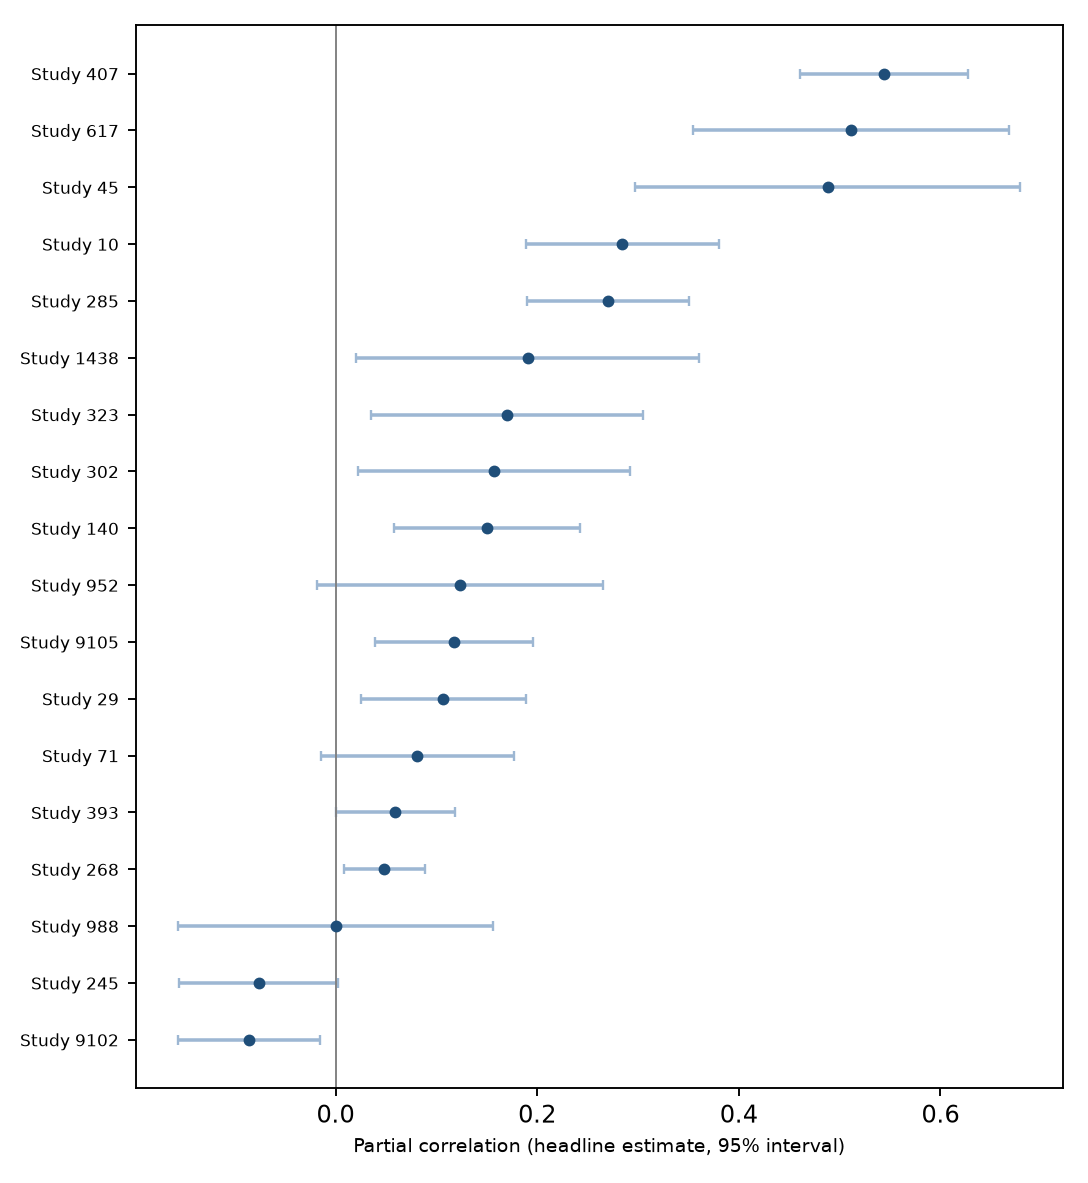
\includegraphics[width=0.62\textwidth]{fig_forest.png}
\caption{Headline partial correlations by study (95\% intervals).}\label{fig:forest}
\end{figure}

\begin{table}[ht]\centering\small
\caption{Moderator meta-regression of partial correlations (125 estimates, 20 papers, standard errors clustered by paper).}\label{tab:mra}
\begin{tabular}{@{}lrrr@{}}\toprule
Moderator & Coefficient & Clustered SE & p\\\midrule
Constant & 0.067 & 0.052 & 0.20\\
Low- or middle-income sample & 0.068 & 0.078 & 0.38\\
System or difference GMM & 0.163 & 0.098 & 0.10\\
Mobile (relative to general ICT) & 0.024 & 0.057 & 0.67\\
Internet or broadband (relative to general ICT) & $-0.066$ & 0.082 & 0.42\\\bottomrule
\end{tabular}\end{table}

Table~\ref{tab:mra} shows no moderator that is distinguishable from zero. In the first run (103 estimates, 18 papers), GMM estimates were 0.16 lower in partial correlation than other methods ($p<0.01$) and internet estimates 0.14 higher ($p=0.09$). Adding the 22 estimates of two studies (9102, an internet-use panel with a growth outcome, and 9105, an instrumental-variable study with an ICT index) turned the GMM coefficient to $+0.16$ ($p=0.10$) and the internet coefficient to $-0.07$. A moderator whose sign changes when two studies are added is not a finding, and the earlier reading that GMM estimates are lower, which looked like support for reverse causation inflating simpler estimates, cannot be maintained; H4 therefore receives no support from the meta-regression. The low- or middle-income indicator is not significant either; 7 papers (23 estimates) come from such samples, against 18 papers and 102 estimates for high-income or mixed samples (mean partial correlation 0.155 against 0.112, unweighted; in the first run the gap was the other way, 0.031 against 0.123). The FAT-PET slope on the standard error is now 1.17 ($p=0.30$) with a bias-corrected intercept of 0.056 ($p=0.36$), and the PEESE intercept is 0.093 ($p=0.06$); in the first run the slope was 1.91 ($p=0.06$) and the corrected values 0.005 and 0.064. The evidence of selective reporting is therefore weaker than in the first run, but the corrected effects (0.06 to 0.09) remain well below the uncorrected 0.17 (Figure~\ref{fig:funnel}). The pooled estimate is stable to the degrees-of-freedom assumption (0.165 to 0.172 for 0, 5 and 20 regressors).

\emph{Sensitivity analyses.} Dropping each study in turn moves the pooled partial correlation between 0.141 and 0.184, so no single study drives the result. Excluding the studies rated critical gives 0.150 (17 papers, 95\% CI 0.072 to 0.228), and excluding one of the two studies that share authors, panel and index (323) gives 0.169. Only one paper with a usable headline estimate was rated at moderate risk of bias, so a restriction to moderate-risk studies is not possible. Restricting to the 9 studies whose design includes an identification strategy beyond controls (internal or external instruments, lagged regressors or a timing design) gives a \emph{higher} pooled value of 0.207 (95\% CI 0.144 to 0.270, $I^2=63\%$), not a lower one. Neither the estimate-level GMM indicator nor the study-level restriction therefore shows that better identification lowers the association. Units differ across studies, and GMM estimates in these studies are often short-run effects of levels on growth rates, which may account for part of the differences.

\begin{figure}[ht]\centering
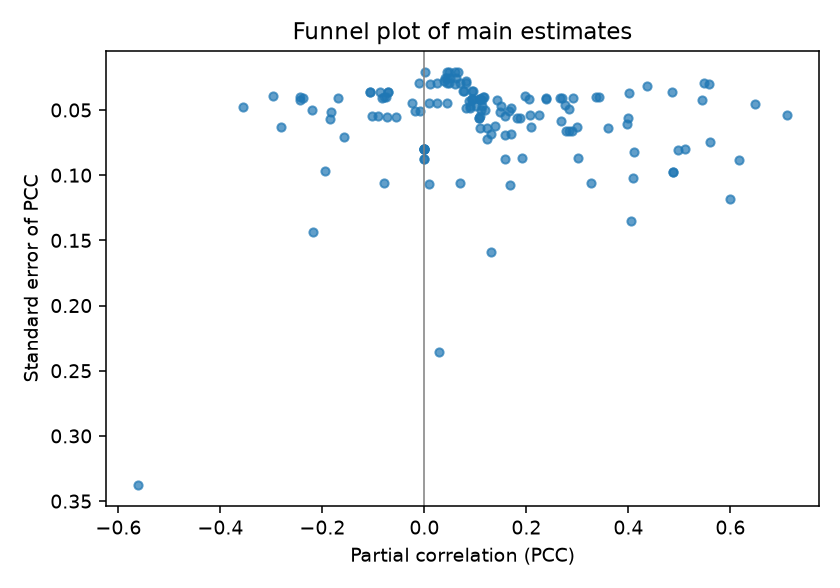
\includegraphics[width=0.58\textwidth]{../review/figures/funnel.png}
\caption{Funnel plot of main estimates (partial correlation against its standard error).}\label{fig:funnel}
\end{figure}

\subsection{Exploratory analyses of additional questions}
\emph{Measurement, outcome form and period.} Adding single variables to the meta-regression, composite-index exposures show a partial correlation 0.05 higher than single indicators (SE 0.09, $p=0.58$) and growth-rate outcomes 0.03 lower than level outcomes (SE 0.10, $p=0.76$); neither is distinguishable from zero, and both rest on between-paper contrasts because few papers contribute both kinds. Later samples show lower partial correlations ($-0.013$ per year of sample midyear, SE 0.008, $p=0.13$), which would be about $-0.13$ per decade. This is not significant, is partly confounded with the shift to GMM in recent studies, and is a hypothesis about diminishing returns, not a finding.

\emph{Design and income coverage.} Studies that list a low-income economy were not more likely to lack an identification strategy (9 of 24, 38\%, against 30 of 53, 57\%; Fisher $p=0.14$) or to be rated at higher risk of bias (moderate risk: 3 of 24 against 6 of 53, $p=1.00$). We therefore find no evidence that weaker designs cluster where low-income economies are sampled, although the comparison has little power. The test of whether study quality goes with a positive direction for output has almost none: only 2 of the 44 output studies were rated at moderate risk of bias, and all family-1 results are positive in 1 of those 2 against 10 of 42 other studies (Fisher $p=0.44$).

\emph{Enabling conditions.} Of the 153 heterogeneity entries, 119 are moderation tests. Human capital is tested in 14 studies (amplifies the effect in 8, dampens it in 3, mixed in 4), income group in 24 (27 entries: richer or higher-income group larger in 8, smaller in 5, mixed in 7, no difference in 5, unclear in 2), infrastructure or connectivity in 9 (5 amplify, 2 dampen), institutions or governance in 8 (3 amplify, 2 dampen, 4 mixed), trade openness in 6 (3 amplify, 2 dampen), financial development in 5 and sector structure in 8 (6 mixed). A second reader agreed with the moderator type in 86\% of a 28-entry sample drawn before the six latest studies were added (kappa 0.83) but with the direction in only 71\% (kappa 0.64), so the direction counts are indicative only. Amplification is the commonest finding for human capital and infrastructure, which is consistent with, but does not show, conditional returns (H2).

\emph{Thresholds.} The studies state 23 thresholds or split points in 17 studies, for the human-capital index, digital maturity, internet penetration, trade openness, private credit and others. They are in different units, rest on one study each and cannot be pooled. Where two studies address the same variable they do not give comparable values.

\emph{Evidence gaps.} Figure~\ref{fig:gap} shows that low-income economies are listed in 15 of 44 output studies, 3 of 14 labour-market studies, 2 of 11 distribution studies and 2 of 6 resource-cost studies. High-income economies are listed in 29 of 44 output studies and 11 of 14 labour-market studies. The historical-wave and AI streams look alike on income-group comparison (44\% against 40\%) but differ on risk of bias (critical in 8\% against 27\%) and first sample year (median 2000 against 2012); the AI stream lists a low-income economy in 2 of 15 studies against 22 of 62 (Fisher $p=0.13$).

\begin{figure}[ht]\centering
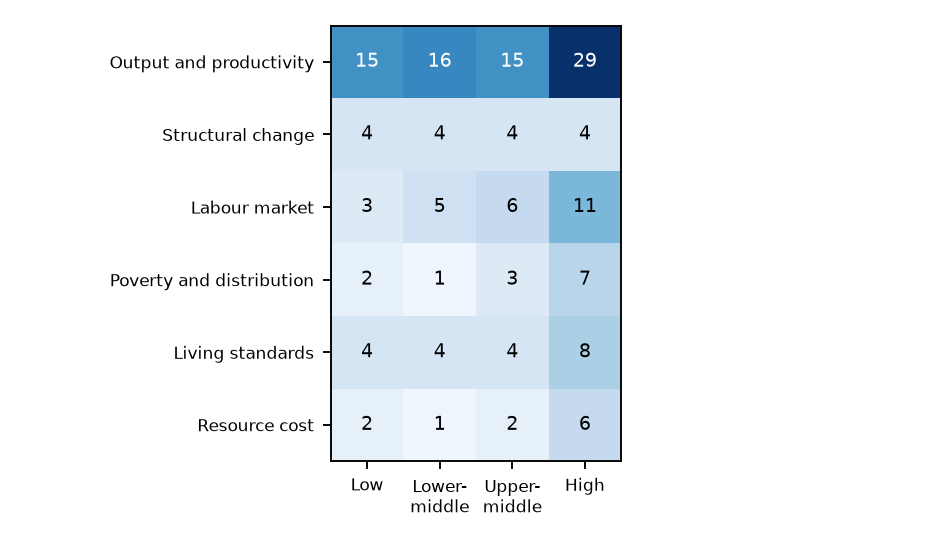
\includegraphics[width=0.58\textwidth]{fig_gap.png}
\caption{Evidence-gap map: studies per outcome family by income groups listed in the sample (a study counts in each group it lists; studies that do not state coverage are not shown).}\label{fig:gap}
\end{figure}

\section{Results of the macro-panel analysis}\label{sec:panel}
\subsection{Mobile adoption and growth by income group (A1, A2)}
Table~\ref{tab:panel} shows that a 10-subscription increase in mobile adoption per 100 people goes with higher annual growth in all four income groups over the same five-year period. The association is largest in lower-middle income economies (0.47 percentage points, 95\% CI 0.16 to 0.77) and about 0.16 in upper-middle and high-income economies; the low-income estimate (0.36) is imprecise (CI $-0.05$ to 0.76, 20 economies). With country fixed effects, the lower-middle estimate remains (0.36, $p=0.03$), and the others move toward 0.13 to 0.20. Extending the sample to 2023 gives the same pattern (lower-middle 0.34, $p<0.01$; upper-middle 0.05, not significant; Appendix Table~\ref{tab:a1m23}).

The predetermined specification, which uses the previous period's change, does not reproduce this pattern: the association is positive only in lower-middle income economies (0.26, $p=0.02$), near zero in upper-middle, and negative in low-income ($-0.38$, $p=0.13$) and high-income ($-0.16$, $p=0.01$) economies, and negative in every income group for internet use (Appendix Table~\ref{tab:a2net}). The contemporaneous associations therefore partly reflect growth driving adoption or shared shocks, and they should not be read as a payoff to adoption. Results for fixed broadband rest on extrapolation from very few observations and are not interpreted (Appendix Table~\ref{tab:a1bb}).

\begin{table}[ht]\centering\small
\caption{Mobile adoption and annual GDP-per-capita growth by income group: change in annual growth (percentage points) per +10 subscriptions per 100 people, five-year periods 1995--2019 (95\% CI; standard errors clustered by country).}\label{tab:panel}
\begin{tabular}{@{}lrrr@{}}\toprule
Income group & Economies & Same period (A1) & Previous period (A2)\\\midrule
Low & 20 & 0.36 [$-0.05$, 0.76] & $-0.38$ [$-0.86$, 0.11]\\
Lower-middle & 42 & 0.47 [0.16, 0.77] & 0.26 [0.03, 0.49]\\
Upper-middle & 51 & 0.16 [0.04, 0.28] & 0.01 [$-0.15$, 0.16]\\
High & 64 & 0.16 [0.05, 0.26] & $-0.16$ [$-0.28$, $-0.03$]\\\bottomrule
\end{tabular}\end{table}

\subsection{Dose-response and differences inside low-income economies (A3, A6)}
Across baseline adoption levels, the association is largest where adoption was below 10 per 100 (0.41) and smaller at 40 to 80 (0.18); it is not monotone, since it is 0.27 above 80 per 100. For low and lower-middle income economies the point estimate above 80 per 100 is the largest (1.37) but imprecise (95\% CI $-0.01$ to 2.74, 35 observations; Appendix Table~\ref{tab:a3}). Inside low and lower-middle income economies, none of initial secondary enrolment, electricity access, private credit or initial income significantly changed the association (all $p>0.19$; Appendix Table~\ref{tab:a6}); the intervals are wide, and a standard-deviation change in a moderator could change the association by about 0.3 percentage points in either direction.

\subsection{Event study around mobile takeoff (A4b)}
The first event-study design, stacked cohorts with controls that adopt more than ten years later or never, was not interpretable (Section~\ref{sec:methods}, Appendix~\ref{app:amend}): nearly every economy crosses the threshold in the window, only 7 clean controls existed for the low and lower-middle income group, and that group showed a pre-trend of 12 log points. The replacement design compares each cohort with economies not yet treated at each horizon and adjusts for initial income and earlier growth. It passes the pre-trend rule in all four samples when the takeoff threshold is 10 subscriptions per 100 (mean placebo effect between $-0.9$ and $0.6$ log points, all intervals including zero; Table~\ref{tab:event}).

\begin{table}[ht]\centering\small
\caption{Event study around the year mobile subscriptions reach 10 per 100 people: effect on log GDP per capita ($\times100$) relative to the year before takeoff and to economies not yet treated (95\% bootstrap interval, 400 draws). Pre-trend: mean of the placebo effects at $-5$ to $-2$ years.}\label{tab:event}
\begin{tabular}{@{}lrlll@{}}\toprule
Sample & Treated & Pre-trend & Effect at +5 years & Effect at +10 years\\\midrule
All economies & 178 & $-0.0$ [$-0.6$, 0.4] & 13.5 [0.6, 36.5] & 47.8 [$-12.5$, 149.1]\\
Low and lower-middle & 66 & 0.6 [$-0.6$, 1.6] & $-5.9$ [$-18.6$, 31.9] & not estimable\\
Upper-middle & 56 & $-0.9$ [$-2.0$, 0.3] & 11.9 [$-8.0$, 46.7] & 12.2 [$-70.1$, 118.6]\\
High & 56 & $-0.4$ [$-1.2$, 0.5] & 19.1 [6.2, 36.7] & 53.8 [4.2, 152.6]\\\bottomrule
\end{tabular}\end{table}

\begin{figure}[ht]\centering
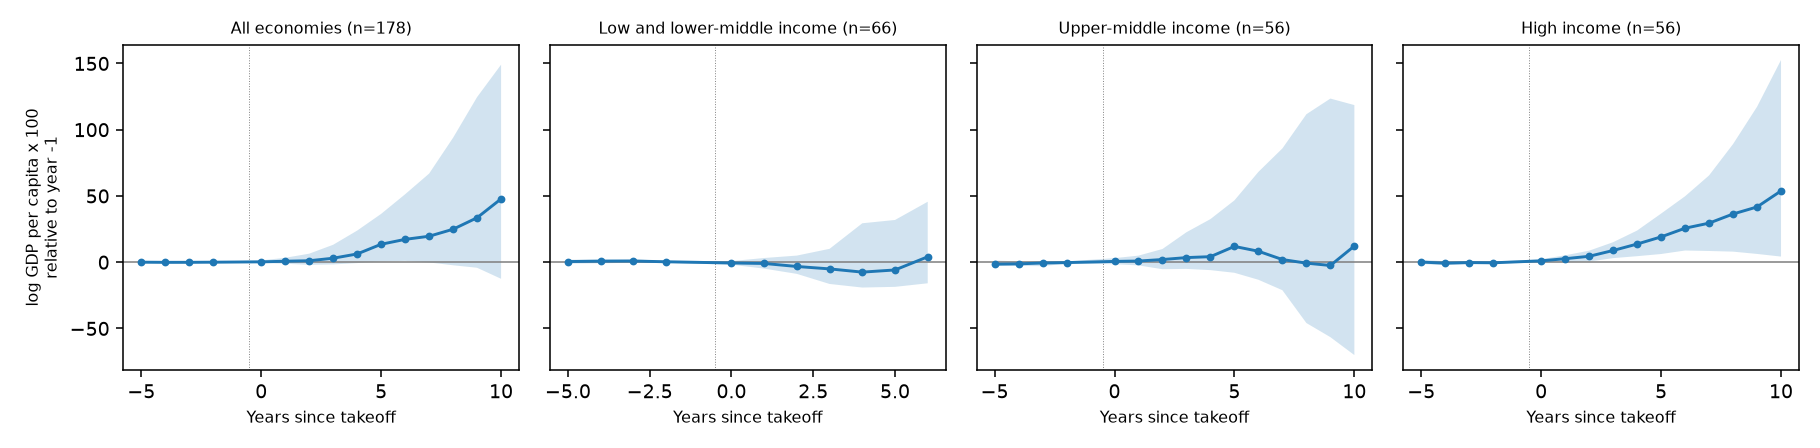
\includegraphics[width=\textwidth]{fig_event.png}
\caption{Event-study estimates by income group (takeoff at 10 mobile subscriptions per 100; shaded: 95\% bootstrap interval). The low and lower-middle panel stops at six years because fewer than eight not-yet-treated economies exist at longer horizons.}\label{fig:event}
\end{figure}

Economies that reach 10 subscriptions per 100 earlier have higher GDP per capita five years later than comparable economies that reach it later, by about 14 log points (95\% CI 0.6 to 36.5). The difference is distinguishable from zero only for high-income economies (19 log points, CI 6.2 to 36.7); the interval for low and lower-middle income economies, $-18.6$ to $+31.9$, is wide enough to contain effects of either sign and of the high-income size. Magnitudes at ten years (about 48 log points overall) are implausibly large for an effect of mobile telephony alone. They mainly show that economies reaching the threshold early are on different growth paths from those reaching it later, in ways initial income and earlier growth do not capture, and that at long horizons only the earliest cohorts contribute. The results are similar with a threshold of 25 per 100 (high income: 15.7 at five years, CI 6.5 to 28.8; low and lower-middle: $-7.5$, CI $-17.6$ to 13.3). With a threshold of 50, the pooled sample and the upper-middle sample fail the pre-trend rule and are not interpreted; the low and lower-middle estimate is 4.3 (CI $-10.7$ to 13.9) and the high-income estimate 8.9 (CI $-0.8$ to 20.8) (Appendix Tables~\ref{tab:es25} and~\ref{tab:es50}).

\emph{Outcomes beyond income.} For samples that pass the pre-trend rule, life expectancy is about 0.9 years higher five years after takeoff in the pooled sample (CI 0.1 to 1.7) and 0.8 years in high-income economies (CI 0.0 to 1.5), with a larger but imprecise estimate for low and lower-middle income economies (2.6 years, CI $-0.5$ to 6.4). Under-5 mortality is 15 log points lower in low and lower-middle income economies (CI $-26.0$ to 1.0). Unemployment and the agriculture share fail the pre-trend rule in most samples, and electricity use is not distinguishable from zero (Appendix Table~\ref{tab:essec}). These outcomes have strong secular trends, so we read these as descriptive.

\subsection{Local projections (A7)}
Local projections give a dynamic profile without a binary treatment (Table~\ref{tab:lp}, Figure~\ref{fig:lp}). For lower-middle income economies, a 10-subscription increase over three years is followed by cumulative growth that is higher by 0.41 percentage points after one year and by 2.0 points after six years (CI 0.8 to 3.2), then 1.7 after eight. For upper-middle and high-income economies, the profile is flat, and the high-income point estimate turns slightly negative (cumulative $-0.5$ after eight years, CI $-1.2$ to 0.2). For low-income economies the profile starts positive and turns negative ($-4.3$ after eight years, CI $-9.2$ to 0.6), but the intervals include zero except as noted. The placebo (future adoption against past growth) is close to zero in every group, though with a wide interval for low-income economies ($-0.75$, CI $-2.5$ to 1.0).

\begin{table}[ht]\centering\small
\caption{Local projections: cumulative growth of GDP per capita (percentage points) $h$ years after a +10 change in mobile subscriptions per 100 over the previous three years (95\% CI; country and year fixed effects).}\label{tab:lp}
\begin{tabular}{@{}lrllll@{}}\toprule
Group & Economies & $h=1$ & $h=2$ & $h=4$ & $h=8$\\\midrule
Low & 24 & 0.25 [$-0.08$, 0.58] & 0.34 [$-0.35$, 1.04] & $-0.44$ [$-2.23$, 1.35] & $-4.31$ [$-9.19$, 0.57]\\
Lower-middle & 47 & 0.41 [0.11, 0.71] & 0.76 [0.25, 1.27] & 1.51 [0.69, 2.33] & 1.69 [0.32, 3.07]\\
Upper-middle & 58 & $-0.00$ [$-0.21$, 0.21] & 0.10 [$-0.19$, 0.38] & 0.22 [$-0.45$, 0.88] & 0.17 [$-0.99$, 1.34]\\
High & 74 & 0.08 [$-0.04$, 0.19] & 0.06 [$-0.16$, 0.29] & $-0.06$ [$-0.48$, 0.35] & $-0.51$ [$-1.23$, 0.20]\\\bottomrule
\end{tabular}\end{table}

\begin{figure}[ht]\centering
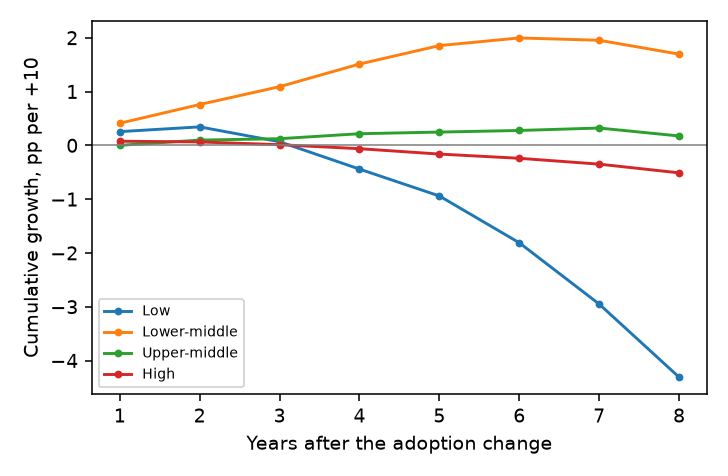
\includegraphics[width=0.6\textwidth]{fig_lp.png}
\caption{Local-projection profiles by income group.}\label{fig:lp}
\end{figure}

\subsection{Consistency across designs}
Table~\ref{tab:designs} summarises which income group shows a positive association under each design. No group is positive under all four. Lower-middle income economies are positive under three (A1, A2, local projections); under the event study they are pooled with low-income economies and the pooled estimate is null with a negative point estimate. High-income economies are positive under the same-period regression and the event study, but flat or negative under the predetermined regression and the local projections. Upper-middle economies are positive only in the same-period regression. Low-income economies are never significantly positive. We conclude that the panel analysis does not support a statement that richer or poorer economies gain more; the answer depends on the design, which is the same message as in the reviewed studies.

\begin{table}[ht]\centering\small
\caption{Direction and significance of the association between mobile adoption and GDP per capita growth, by design and income group (+ positive and significant at 5\%, $-$ negative and significant, 0 not significant; sign of the point estimate in parentheses).}\label{tab:designs}
\begin{tabular}{@{}lllll@{}}\toprule
Design & Low & Lower-middle & Upper-middle & High\\\midrule
A1 same period & 0 (+) & + & + & +\\
A2 previous period & 0 ($-$) & + & 0 (+) & $-$\\
Event study (+5 years) & \multicolumn{2}{c}{0 ($-$), low and lower-middle pooled} & 0 (+) & +\\
Local projections ($h=6$) & 0 ($-$) & + & 0 (+) & 0 ($-$)\\\bottomrule
\end{tabular}\end{table}



\section{Discussion}\label{sec:discussion}

\subsection{What the evidence supports}
Four points stand out across the review and the panel analysis. First, the central estimate of the association between ICT-type adoption and output is positive but modest and very heterogeneous across studies (H1), and it shrinks when we allow for small-study bias. We find no support for H4: the GMM indicator changed sign when two studies were added, and restricting to studies with an identification strategy raises the pooled value. A partial correlation of 0.17 means that adoption explains a few percent of the residual variation in output, and the bias-corrected estimates are smaller still.

Second, returns look conditional on human capital, financial depth, governance and infrastructure (H2). Amplification is the commonest finding when authors test these conditions. This agrees with the long-run diffusion evidence that the intensity of use, rather than arrival, drives divergence \cite{comin2018}, although the studies we synthesise cannot show that changing a moderator would change the return. The threshold results, such as a human-capital index below which the effect of the digital economy is negative in Africa, suggest that the conditions are not marginal but may bind. That reading needs replication, since each threshold comes from one study.

Third, the question of whether poorer or richer economies gain more cannot be answered from the reviewed evidence (H3). The comparisons that exist are few, mostly informal and often from weak designs, and low-income economies are rarely sampled. The measured association in the studies leans toward richer samples, but design differences could produce that lean.

Fourth, the timing of effects matters, but few studies examine it (H5). A study with a five-year lag found a positive effect where the contemporaneous effect was null. In our own analysis, predetermined and contemporaneous specifications give different pictures; the local projections show gains in lower-middle income economies building over about six years, and the event study shows gains in high-income economies emerging after the third year. Any claim about gains from a technology should state the horizon.

\subsection{Reconciling the review with the panel analysis}
The panel analysis adds a cautious observation. Under a single same-period design, the association between mobile adoption and growth is not smaller in poorer economies: it is largest in lower-middle income economies. This runs against the lean in the reviewed studies toward larger measured gains in richer samples. But the picture depends on the design: the event study finds a distinguishable gain only for high-income economies, and local projections only for lower-middle income economies, so the panel analysis does not settle which group gains more either. The two sources differ in technology (the panel covers mobile subscriptions only), in outcome (growth of GDP per capita) and in design (we use one specification for all groups, while the studies use different specifications by group), so they are not in direct conflict. The predetermined version does not reproduce the association, so we do not take it as evidence that poorer economies gain more. The honest summary is that the two sources do not agree on a difference by income, and neither identifies a causal effect.

\subsection{AI}
The evidence on AI is too thin and short to be put next to the evidence on earlier waves (H6). The few studies that exist show patterns similar to those for ICT where they test them: larger measured effects in richer economies and in high-skill occupations. But the exposure measures are indices of readiness or occupational exposure, the panels are short, 27\% of the AI studies are rated critical, and only two list a low-income economy. A comparison with earlier technologies would require evidence on realised use, which none of the included studies has.

\subsection{Implications}
For policy, the safest reading is that digital investment is unlikely to pay off equally everywhere and that complementary capabilities matter. The review does not support statements of the form that a given income group should expect a given payoff. Three practical points follow. Evaluations of digital programmes should report effects at several horizons, because contemporaneous estimates can mislead. Programmes in low-income settings should be paired with, or at least monitored against, the complements the literature highlights, such as skills, electricity and finance. And claims about AI should be treated as provisional until studies with measures of realised use and credible designs appear.

\subsection{Research agenda}
For research, the main need is identification for developing and low-income economies, with instruments or timing designs of the kind used for submarine cables \cite{hjort2019}, and for AI, measures of realised use rather than readiness. Second, studies should report group-specific effects with a test of the difference, which most studies do not. Third, a registered, two-reviewer systematic review with Scopus, Web of Science and a complete Google Scholar search would reduce the selection concerns listed below. Fourth, the thresholds reported in single studies should be tested for replication across samples.

\section{Limitations}\label{sec:limits}

\begin{itemize}[leftmargin=1.4em,itemsep=2pt]
\item \textbf{Selection.} Only studies with a free or supplied full text were read: about 140 of the 247 records sent to full-text assessment are unread, and paywalled studies are over-represented among them. Records from four venues the author judged unreliable were skipped. Search covered OpenAlex, Crossref and NBER, plus the first page of one Google Scholar query; Scopus, Web of Science and EconLit were not run, and the other Google Scholar queries have not been run. The main search had poor recall (9 of 10 first-page Google Scholar results were missing from it), so the review is not exhaustive and its pooled results could shift as studies are added, as they did when two were.
\item \textbf{Single reviewer.} Screening used one assisted reviewer. A blind re-screening of a random sample by a separate model run gave moderate agreement at the abstract stage (79\%, kappa 0.59) and suggests that the screening missed records a careful reader would include (Section~\ref{sec:crosscheck}). Extraction was by machine with a second machine pass and then checked on a random sample by the author by hand; the rest of the data has not been checked by a person, and no second human reviewer verified it independently.
\item \textbf{Registration.} The protocol was not registered before the search. The certainty of the evidence was not graded (GRADE was not applied).
\item \textbf{Design quality.} No study has low risk of bias; most treat adoption as exogenous. We report associations, not causal effects. First-pass risk-of-bias ratings are used; nine ratings would change under the second pass, and the blind re-extraction agreed on the overall rating for only 11 of 16 studies, so the ratings are subjective.
\item \textbf{Counting.} Direction counts are not weighted by size or quality and are not effect sizes. Study-level income comparisons mix World Bank income groups, regions and developed-developing splits.
\item \textbf{Meta-regression.} Eighteen papers with a headline estimate (20 with any usable estimate); the moderator estimates changed sign when two studies were added, so they are unstable, and the clustered standard errors are optimistic. Partial correlations rely on an assumed degrees of freedom. Composite indices, levels and growth outcomes, and conditional main effects are mixed in one analysis despite exclusions. Two Asian studies (302 and 323) share authors, panel and index and are not independent. The sample is not a census, and the low- and middle-income group is small.
\item \textbf{Language and period.} English only, 1995 onward.
\item \textbf{Macro-panel analysis.} The World Bank panel analysis gives conditional associations only. Income groups use the current classification; the planned check with initial income was not run; CO2 emissions could not be retrieved. Roughly forty estimates were reported without correction for multiple testing.
\end{itemize}

\section{Conclusion}\label{sec:conclusion}

Across 77 studies, ICT-type adoption is usually associated with higher output, but the association is modest, strongly heterogeneous, shrinks under a correction for small-study bias, is not lower in studies with credible identification, and is reported to be conditional on human capital, financial depth, governance and infrastructure. Whether rich or poor economies gain more is not established, and the evidence on AI is too thin to compare with earlier waves. A World Bank panel analysis finds that mobile adoption goes with faster growth in every income group in a same-period regression, most strongly in lower-middle income economies, but the pattern changes with the design (a staggered event study finds a gain only for high-income economies, and local projections only for lower-middle income economies), so without a causal design it is not a payoff. The search missed many relevant studies and adding two of them changed the moderator results, so those results should be treated as provisional. Credible identification for low- and middle-income economies and realised-use measures for AI are the main gaps.

\section*{Declarations}
\small
\noindent\textbf{Data and code availability.} The protocol, search and screening logs, extraction database, second-pass verification files, meta-regression inputs, World Bank panel and all code are in the project repository: \url{https://github.com/vinhqdang/Journal-of-Economy-and-Technology}. Full-text PDFs are not shared for copyright reasons.\\
\textbf{Ethics.} Not applicable; the review uses published studies and public statistics only.\\
\textbf{Author contributions (CRediT).} \todo{author to complete}\\
\textbf{Conflict of interest.} \todo{author to complete}\\
\textbf{Funding.} No external funding was declared in the protocol. \todo{author to confirm}\\
\textbf{Use of AI tools.} Generative AI tools were used to support this work: to polish the writing, to assist with screening records and extracting data from the included studies (described in the Methods), and to help write and run analysis code. The ideas, the research question and direction, and the choice of methods and algorithms are the author's own. The author reviewed the AI-assisted output and takes full responsibility for the content of this paper.\\
\textbf{Registration.} \todo{OSF registration pending}

\normalsize
\begin{thebibliography}{99}\small
\bibitem{roller2001} L.-H. R\"oller and L. Waverman (2001). Telecommunications infrastructure and economic development: a simultaneous approach. \emph{American Economic Review} 91(4), 909--923. doi:10.1257/aer.91.4.909.
\bibitem{comin2010} D. Comin and B. Hobijn (2010). An exploration of technology diffusion. \emph{American Economic Review} 100(5), 2031--2059. doi:10.1257/aer.100.5.2031.
\bibitem{comin2018} D. Comin and M. Mestieri (2018). If technology has arrived everywhere, why has income diverged? \emph{American Economic Journal: Macroeconomics} 10(3), 137--178. doi:10.1257/mac.20150175.
\bibitem{jensen2007} R. Jensen (2007). The digital provide: information (technology), market performance, and welfare in the South Indian fisheries sector. \emph{Quarterly Journal of Economics} 122(3), 879--924. doi:10.1162/qjec.122.3.879.
\bibitem{aker2010} J. C. Aker and I. M. Mbiti (2010). Mobile phones and economic development in Africa. \emph{Journal of Economic Perspectives} 24(3), 207--232. doi:10.1257/jep.24.3.207.
\bibitem{hjort2019} J. Hjort and J. Poulsen (2019). The arrival of fast internet and employment in Africa. \emph{American Economic Review} 109(3), 1032--1079. doi:10.1257/aer.20161385.
\bibitem{autor2003} D. H. Autor, F. Levy and R. J. Murnane (2003). The skill content of recent technological change: an empirical exploration. \emph{Quarterly Journal of Economics} 118(4), 1279--1333. doi:10.1162/003355303322552801.
\bibitem{acemoglu2019} D. Acemoglu and P. Restrepo (2019). Automation and new tasks: how technology displaces and reinstates labor. \emph{Journal of Economic Perspectives} 33(2), 3--30. doi:10.1257/jep.33.2.3.
\bibitem{cohen1990} W. M. Cohen and D. A. Levinthal (1990). Absorptive capacity: a new perspective on learning and innovation. \emph{Administrative Science Quarterly} 35(1), 128--152. doi:10.2307/2393553.
\bibitem{dedrick2003} J. Dedrick, V. Gurbaxani and K. L. Kraemer (2003). Information technology and economic performance. \emph{ACM Computing Surveys} 35(1), 1--28. doi:10.1145/641865.641866.
\bibitem{prisma2020} M. J. Page et al. (2021). The PRISMA 2020 statement: an updated guideline for reporting systematic reviews. \emph{BMJ} 372, n71. doi:10.1136/bmj.n71.
\bibitem{prismap} D. Moher et al. (2015). Preferred reporting items for systematic review and meta-analysis protocols (PRISMA-P) 2015 statement. \emph{Systematic Reviews} 4, 1. doi:10.1186/2046-4053-4-1.
\bibitem{swim} M. Campbell et al. (2020). Synthesis without meta-analysis (SWiM) in systematic reviews: reporting guideline. \emph{BMJ} 368, l6890. doi:10.1136/bmj.l6890.
\bibitem{robinsi} J. A. C. Sterne et al. (2016). ROBINS-I: a tool for assessing risk of bias in non-randomised studies of interventions. \emph{BMJ} 355, i4919. doi:10.1136/bmj.i4919.
\bibitem{stanley2012} T. D. Stanley and H. Doucouliagos (2012). \emph{Meta-Regression Analysis in Economics and Business}. Routledge. doi:10.4324/9780203111710.
\bibitem{stanley2014} T. D. Stanley and H. Doucouliagos (2014). Meta-regression approximations to reduce publication selection bias. \emph{Research Synthesis Methods} 5(1), 60--78. doi:10.1002/jrsm.1095.
\bibitem{dersimonian1986} R. DerSimonian and N. Laird (1986). Meta-analysis in clinical trials. \emph{Controlled Clinical Trials} 7(3), 177--188. doi:10.1016/0197-2456(86)90046-2.
\bibitem{callaway2021} B. Callaway and P. H. C. Sant'Anna (2021). Difference-in-differences with multiple time periods. \emph{Journal of Econometrics} 225(2), 200--230. doi:10.1016/j.jeconom.2020.12.001.
\bibitem{sun2021} L. Sun and S. Abraham (2021). Estimating dynamic treatment effects in event studies with heterogeneous treatment effects. \emph{Journal of Econometrics} 225(2), 175--199. doi:10.1016/j.jeconom.2020.09.006.
\bibitem{dechaisemartin2020} C. de Chaisemartin and X. D'Haultf\oe uille (2020). Two-way fixed effects estimators with heterogeneous treatment effects. \emph{American Economic Review} 110(9), 2964--2996. doi:10.1257/aer.20181169.
\bibitem{jorda2005} \`O. Jord\`a (2005). Estimation and inference of impulse responses by local projections. \emph{American Economic Review} 95(1), 161--182. doi:10.1257/0002828053828518.
\end{thebibliography}

\appendix
\section{Included studies}\label{app:studies}
{\footnotesize
\begin{longtable}{@{}r r p{4.9cm} p{1.5cm} r l p{3.7cm}@{}}
\caption{Studies included in the synthesis (n = 71). Authors are not listed because the extraction database does not store them; the DOI identifies each record. n.r. = not reported. RoB = overall risk of bias in the first-pass rating (moderate, serious, critical); no study was rated low.}\label{tab:included}\\
\toprule ID & Year & Title & Technology & Econ. & RoB & DOI \\ \midrule \endfirsthead
\toprule ID & Year & Title & Technology & Econ. & RoB & DOI \\ \midrule \endhead
\bottomrule \endfoot
10 & 2020 & Financial inclusion, information and communication technology diffusion, and economic growth: a panel data analysis & ICT, Mobile, Internet & 41 & serious & \url{https://doi.org/10.1080/02681102.2020.1734770} \\
29 & 2019 & The Internet of Things and economic growth in a panel of countries & ICT, Mobile, Internet & 82 & serious & \url{https://doi.org/10.1080/10438599.2019.1695941} \\
45 & 2024 & Financial inclusion through digitalization and economic growth in Asia-Pacific countries & ICT, Mobile, Internet & 30 & serious & \url{https://doi.org/10.1016/j.irfa.2024.103596} \\
57 & 2020 & Nexus between energy consumption, information and communications technology, and economic growth: An enquiry into emerging Asian countries & ICT, Mobile, Internet & 10 & serious & \url{https://doi.org/10.1002/pa.2172} \\
68 & 2022 & Enhancing human development in developing regions: Do ICT and transport infrastructure matter? & ICT, Mobile, Internet & 79 & serious & \url{https://doi.org/10.1016/j.techfore.2022.121725} \\
71 & 2022 & The ICT, financial development, energy consumption and economic growth nexus in MENA countries: dynamic panel CS-ARDL evidence & ICT, Mobile, Internet & 11 & serious & \url{https://doi.org/10.1080/00036846.2022.2096861} \\
88 & 2005 & Does the digital divide matter? The role of information and communication technology in cross-country level and growth estimates & ICT, Mobile, Internet & 94 & serious & \url{https://doi.org/10.1080/1043859042000304043} \\
108 & 2024 & New technologies and jobs in Europe & AI & 16 & moderate & \url{https://doi.org/10.1093/epolic/eiae058} \\
126 & 2023 & Job creation and destruction in the digital age: Assessing heterogeneous effects across European Union countries & ICT & 27 & moderate & \url{https://doi.org/10.1016/j.econmod.2023.106405} \\
138 & 2023 & Empirical Analysis of Inclusive Growth, Information and Communication Technology Adoption, and Institutional Quality & ICT, Mobile, Internet & 193 & serious & \url{https://doi.org/10.3390/economies11040124} \\
140 & 2015 & What are the drivers of total factor productivity in the European Union? & ICT & 17 & serious & \url{https://doi.org/10.1080/10438599.2015.1067007} \\
162 & 2024 & Impact of digitization on carbon productivity: an empirical analysis of 136 countries & Mobile, Internet & 136 & serious & \url{https://doi.org/10.1038/s41598-024-55848-2} \\
174 & 2025 & Artificial intelligence and global carbon inequality: Addressing the challenges and opportunities for SDG 10, SDG 12, and SDG 13 & AI & 67 & serious & \url{https://doi.org/10.1016/j.gsf.2025.102072} \\
217 & 2021 & Does digital financial inclusion moderate or exacerbate output volatility? & Mobile & 40 & serious & \url{https://doi.org/10.1080/13504851.2021.1963400} \\
239 & 2018 & What drives labor market polarization in advanced countries? The role of China and technology & ICT & 19 & serious & \url{https://doi.org/10.1093/icc/dty063} \\
245 & 2023 & The impact of the digital economy on green total factor productivity in Belt and Road countries: the mediating role of energy transition & ICT, Internet & 40 & serious & \url{https://doi.org/10.3389/fenvs.2023.1213961} \\
268 & 2023 & Informality and aggregate labor productivity growth: Does ICT moderate the relationship? & ICT, Internet & 118 & serious & \url{https://doi.org/10.1016/j.telpol.2023.102681} \\
269 & 2024 & Economic growth and the proliferation of ICT infrastructures: which causes the other? & ICT, Mobile, Internet & 41 & serious & \url{https://doi.org/10.1080/1331677x.2024.2310100} \\
276 & 2025 & Does artificial intelligence help in improving human capital based educational development? Evidence from 29 countries & AI & 29 & serious & \url{https://doi.org/10.1016/j.techsoc.2025.103004} \\
278 & 2024 & Towards ICT diffusion and trade liberalisation on inclusive growth in Sub-Saharan Africa & ICT, Mobile, Internet & 48 & serious & \url{https://doi.org/10.1007/s10668-023-04355-x} \\
285 & 2022 & ICT and Economic Growth in EU: A macro Level Comparison of Estimated ICT Output Elasticities & ICT & 27 & moderate & \url{https://doi.org/10.1080/1097198x.2022.2094182} \\
302 & 2013 & Does ICT Participate in Economic Convergence among Asian Countries: Evidence from Dynamic Panel Data Model & ICT, Mobile, Internet & 24 & serious & \url{https://doi.org/10.12948/issn14531305/17.2.2013.01} \\
320 & 2022 & The Effect of Technology Adoption on Financial Inclusion: A Cross-country Panel Analysis between China and Nigeria & Mobile, Internet & 20 & serious & \url{https://doi.org/10.24018/ejbmr.2022.7.2.1314} \\
321 & 2024 & Information and communication technology and labour productivity growth: a production-frontier approach & ICT & 24 & serious & \url{https://doi.org/10.1007/s10479-024-05818-8} \\
323 & 2014 & Total Factor Productivity, Demographic Traits and ICT: Empirical Analysis for Asia & ICT, Mobile, Internet & 24 & serious & \url{https://doi.org/10.12948/issn14531305/18.1.2014.01} \\
341 & 2024 & The impact of information and communication technologies on export diversification: Evidence from developing countries & ICT, Mobile, Internet & 110 & moderate & \url{https://doi.org/10.1080/09638199.2024.2419406} \\
358 & 2023 & Digital Divide, Credit Financing and Financial Inclusion: Changing Patterns of Poverty, Employment and Income Inequalities & Mobile, Internet & 148 & serious & n.a. \\
392 & 2018 & TECHNOLOGICAL SOURCES OF ECONOMIC GROWTH IN EUROPE AND THE U.S. & ICT & 10 & serious & \url{https://doi.org/10.3846/20294913.2017.1280557} \\
393 & 2013 & The Determinants of Total Factor Productivity in the EU: Insights from Sectoral Data and Common Dynamic Processes & ICT & 17 & serious & n.a. \\
407 & 2015 & The Role of ICT in the Productivity of Central and Eastern European Countries: Cross-country Comparison & ICT, Internet & 21 & serious & n.a. \\
408 & 2025 & Effects of the digital economy on economic growth in Africa: the role of human capital & ICT, Mobile, Internet & 41 & serious & \url{https://doi.org/10.1080/23322039.2025.2525485} \\
422 & 2024 & Icts And Labour Productivity Nexus In Developing Countries: Evidence From Panel Estimation Approach & ICT, Mobile, Internet & 84 & serious & \url{https://doi.org/10.33736/ijbs.6868.2024} \\
441 & 2024 & Artificial Intelligence Readiness and Employment: A Global Panel Analysis & AI & 78 & critical & \url{https://doi.org/10.24818/18423264/58.4.24.04} \\
442 & 2025 & From Digital Divide to Employment Equity: How Digitalization Affects Women's Involvement in the Workforce in OECD Countries & Mobile, Internet & 22 & critical & \url{https://doi.org/10.17583/generos.15672} \\
448 & 2025 & Unraveling the digital technologies and banking inclusion nexus in Sub Saharan Africa & Mobile, Internet & 45 & serious & \url{https://doi.org/10.1007/s43621-025-01694-9} \\
535 & 2026 & The Economic Value of Agentic AI: A Comparative Analysis of Its Impact on Growth and Business Productivity in Developed and Emerging Economies & AI & 10 & critical & \url{https://doi.org/10.9734/ajrcos/2026/v19i5859} \\
617 & 2003 & Bridging the digital divide: the growth implications of e-commerce for small and developing states & Internet & 205 & critical & n.a. \\
707 & 2026 & Digitalisation and structural change: Evidence from cross-country analysis & Mobile, Internet & 51 & serious & \url{https://doi.org/10.1016/j.jdec.2026.03.003} \\
750 & 2025 & Artificial Intelligence and Labour Markets in Southeast Asia: An Empirical Examination & AI & 1 & serious & \url{https://doi.org/10.46557/001c.132415} \\
755 & 2026 & Artificial intelligence investment and renewable energy for environmental sustainability in ASEAN-5 under the foreign direct investment threshold & AI & 5 & serious & \url{https://doi.org/10.1007/s43621-026-03998-w} \\
802 & 2015 & Differences in Job De-Routinization in OECD Countries: Evidence from PIAAC & ICT & 22 & serious & n.a. \\
803 & 2020 & The Race between Technological Progress and Female Advancement: Changes in Gender and Skill Premia in OECD Countries & ICT & 11 & moderate & n.a. \\
879 & 2026 & AI capability and labor productivity in low- and middle-income countries: An absorptive capacity approach & AI, ICT, Mobile, Internet & 63 & serious & \url{https://doi.org/10.1016/j.technovation.2026.103645} \\
891 & 2026 & Can Artificial Intelligence Drive Sustainable Growth? Empirical Evidence on the AI-Energy-Growth Nexus in Advanced Economies & AI, ICT & 9 & serious & \url{https://doi.org/10.3390/su18052308} \\
913 & 2026 & Estimation of Firm Labour Productivity and Sales Growth from Artificial Intelligence in Sub-Saharan African Countries & AI & 10 & critical & \url{https://doi.org/10.12688/f1000research.179912.1} \\
952 & 2026 & Twin Transition and Labor Informality in Asia-Pacific: Threshold Effects and Income-Group Heterogeneity & ICT, Internet & 17 & serious & \url{https://doi.org/10.3390/economies14090398} \\
957 & 2024 & IMPACT OF ICT ON ECONOMIC GROWTH: CASE OF OECD AND MENA COUNTRIES & ICT, Mobile, Internet & 32 & serious & \url{https://doi.org/10.59671/dga69} \\
988 & 2023 & IMPACT OF DIGITALISATION ON PRODUCTIVITY GROWTH IN EU MEMBER STATES & ICT & 27 & serious & \url{https://doi.org/10.30525/2661-5169/2023-3-2} \\
1013 & 2025 & The Effect of Artificial Intelligence Investments on Economic Development: Panel Data Analysis & AI & 8 & serious & \url{https://doi.org/10.17694/bajece.1802500} \\
1025 & 2005 & Testing the impact of ICT in developed countries during 1980-1995: distributional analysis in Solow's growth accounting framework & ICT & 15 & serious & n.a. \\
1026 & 2026 & The nonlinear link between AI and energy poverty: Empirical evidence from global data & AI & 64 & serious & \url{https://doi.org/10.1016/j.jclepro.2026.148590} \\
1031 & 2025 & Exploring the Moderating impact of ICT Infrastructure on Trade Openness-Sectoral Growth Nexus in Sub-Saharan Africa (SSA) & ICT, Mobile, Internet & 26 & serious & \url{https://doi.org/10.58709/niujhu.v10i3.2267} \\
1192 & 2026 & The Digital Maturity Paradox: The Divergent Impact of Network Readiness and FDI Across Development Tiers & ICT & 121 & critical & \url{https://doi.org/10.3390/economies14080320} \\
1372 & 2024 & The relationship between inequality and poverty in developing countries: mitigating role of virtual social network and internet access in schools & Internet & 57 & serious & \url{https://doi.org/10.1108/ijse-09-2023-0695} \\
1419 & 2017 & Mobile banking usage, quality of growth, inequality and poverty in developing countries & Mobile & 93 & serious & \url{https://doi.org/10.1177/0266666917744006} \\
1428 & 2021 & IMPACT OF MOBILE PHONES AND INTERNET USE ON FINANCIAL INCLUSION: EMPIRICAL EVIDENCE FROM THE EU POST-COMMUNIST COUNTRIES & Mobile, Internet & 11 & serious & \url{https://doi.org/10.3846/tede.2021.14508} \\
1438 & 2021 & Impact of Economic Integration and Information and Communication Technology on Economic Growth for European Union: Dynamic Panel GMM Approach & ICT, Mobile, Internet & 27 & serious & \url{https://doi.org/10.5296/ber.v11i4.19064} \\
1448 & 2023 & The effect of information and communication technology on economic growth high-income countries & ICT, Mobile, Internet & 10 & serious & \url{https://doi.org/10.55493/5002.v13i9.4824} \\
1469 & 2026 & Reducing Gender Inequality in Education in Developing Countries: Do Information and Communication Technologies Matter? & ICT, Mobile, Internet & 64 & serious & \url{https://doi.org/10.1002/sd.71201} \\
1494 & 2026 & Digital transformation and income disparities: A threshold analysis in developing countries & ICT, Mobile, Internet & 45 & serious & \url{https://doi.org/10.1556/032.2025.00183} \\
1526 & 2022 & Artificial Intelligence and Employment: New Cross-Country Evidence & AI & 23 & moderate & \url{https://doi.org/10.3389/frai.2022.832736} \\
1564 & 2025 & The Impact of Artificial Intelligence on Employment: A Panel Data Analysis for Selected Countries & AI & 29 & serious & \url{https://doi.org/10.30784/epfad.1621455} \\
1596 & 2026 & Impact of Generative AI Adoption on Micro and Small Enterprises in Emerging Economies & Other & 3 & critical & \url{https://doi.org/10.64060/ijpssdv2i12} \\
1645 & 2025 & Cryptocurrency Adoption Patterns and Financial Inclusion Outcomes in Emerging Market Economies & Mobile, Internet, Crypto & 15 & critical & \url{https://doi.org/10.71086/iajir/v12i4/iajir1244} \\
1652 & 2025 & Crypto-driven growth: A comparative study of Bitcoin and Ethereum on economic growth for multi-country analysis & Crypto & 14 & critical & \url{https://doi.org/10.32609/j.ruje.11.164511} \\
1670 & 2019 & FINANCIAL INCLUSION, MOBILE PHONE DIFFUSION, AND ECONOMIC GROWTH; EVIDENCE FROM AFRICA & Mobile & 32 & serious & \url{https://doi.org/10.32479/ijefi.8256} \\
1679 & 2022 & The Employment Effects of Mobile Internet in Developing Countries & Mobile, Internet & 14 & moderate & n.a. \\
1713 & 2012 & ICT capital and labour productivity growth: A non-parametric analysis of 14 OECD countries & ICT & 14 & serious & \url{https://doi.org/10.1016/j.telpol.2011.12.012} \\
1759 & 2022 & ICT capital–skill complementarity and wage inequality: Evidence from OECD countries & ICT & 14 & moderate & \url{https://doi.org/10.1016/j.labeco.2022.102151} \\
1798 & 2022 & The role of governance in the effect of the internet on financial inclusion in sub-Saharan Africa & Internet & 42 & serious & \url{https://doi.org/10.2139/ssrn.4315622} \\
9001 & 2019 & The association between mobile phones and the risk of brain cancer mortality: a 25-year cross-country analysis & Mobile & 88 & serious & \url{https://doi.org/10.1111/coep.12456} \\
\end{longtable}
}


\section{Results by outcome family}\label{app:families}
{\scriptsize
\begin{longtable}{@{}r l r l l p{3.6cm} l@{}}
\caption{Studies reporting output and productivity outcomes (n = 53). ``Directions'' counts the study's results in this family: $+$ positive, $-$ negative, 0 null, m mixed. Technology codes as in Table~\ref{tab:included}.}\label{tab:fam1}\\
\toprule ID & Tech. & Econ. & Years & Estimator & Directions & RoB \\ \midrule \endfirsthead
\toprule ID & Tech. & Econ. & Years & Estimator & Directions & RoB \\ \midrule \endhead
\bottomrule \endfoot
10 & ICT, Mobile, Internet & 41 & 2004--2015 & GMM & 20, 5m & serious \\
29 & ICT, Mobile, Internet & 82 & 2010--2017 & FE/RE/OLS & 7+, 10 & serious \\
45 & ICT, Mobile, Internet & 30 & 2014--2021 & FE/RE/OLS & 5+ & serious \\
57 & ICT, Mobile, Internet & 10 & 2000--2017 & ARDL/coint./heterog. panel & 2+, 1$-$, 20, 1m & serious \\
71 & ICT, Mobile, Internet & 11 & 1980--2018 & ARDL/coint./heterog. panel & 3+ & serious \\
88 & ICT, Mobile, Internet & 94 & 1983--1997 & FE/RE/OLS & 4+, 1m & serious \\
140 & ICT & 17 & 1995--2007 & ARDL/coint./heterog. panel & 1+ & serious \\
217 & Mobile & 40 & 2009--2017 & GMM & 5+, 1m & serious \\
245 & ICT, Internet & 40 & 2006--2021 & ARDL/coint./heterog. panel & 3$-$, 2m & serious \\
268 & ICT, Internet & 118 & 1997--2017 & FE/RE/OLS & 3+, 3$-$, 30, 2m & serious \\
269 & ICT, Mobile, Internet & 41 & 2000--2019 & ARDL/coint./heterog. panel & 2+, 10 & serious \\
285 & ICT & 27 & 1996--2016 & FE/RE/OLS & 6+ & moderate \\
302 & ICT, Mobile, Internet & 24 & 2000--2010 & GMM & 2+, 1$-$ & serious \\
321 & ICT & 24 & 1995--2019 & Accounting/DEA/other & 3+, 1$-$, 10, 2m & serious \\
323 & ICT, Mobile, Internet & 24 & 2000--2010 & GMM & 2+ & serious \\
358 & Mobile, Internet & 148 & 2008--2021 & FE/RE/OLS & 1+ & serious \\
392 & ICT & 10 & 1980--2010 & Accounting/DEA/other & 3+, 10 & serious \\
393 & ICT & 17 & 1995--2007 & ARDL/coint./heterog. panel & 3+, 10 & serious \\
407 & ICT, Internet & 21 & 1993--2011 & FE/RE/OLS & 4+, 10, 1m & serious \\
408 & ICT, Mobile, Internet & 41 & 2000--2021 & GMM & 5+, 1$-$ & serious \\
422 & ICT, Mobile, Internet & 84 & 2000--2019 & GMM & 5+, 1m & serious \\
535 & AI & 10 & 2015--2024 & FE/RE/OLS & 7+ & critical \\
617 & Internet & 205 & 2000 & Accounting/DEA/other & 2+ & critical \\
879 & AI, ICT, Mobile, Internet & 63 & 2005--2019 & GMM & 7+, 1m & serious \\
891 & AI, ICT & 9 & 2010--2025 & ARDL/coint./heterog. panel & 1+, 1$-$, 20 & serious \\
913 & AI & 10 & 2007--2024 & FE/RE/OLS & 4+, 20, 2m & critical \\
952 & ICT, Internet & 17 & 2005--2022 & GMM & 2+ & serious \\
957 & ICT, Mobile, Internet & 32 & 2010--2023 & GMM & 3+, 40, 1m & serious \\
988 & ICT & 27 & 2017--2022 & FE/RE/OLS & 2+, 10 & serious \\
1025 & ICT & 15 & 1980--1995 & Accounting/DEA/other & 20, 2m & serious \\
1192 & ICT & 121 & 2023 & FE/RE/OLS & 1+, 1$-$, 10, 1m & critical \\
1419 & Mobile & 93 & 2005--2011 & FE/RE/OLS & 2m & serious \\
1438 & ICT, Mobile, Internet & 27 & 2002--2019 & GMM & 2+, 2m & serious \\
1448 & ICT, Mobile, Internet & 10 & 2001--2020 & FE/RE/OLS & 40 & serious \\
1580 & AI & 122 & 1970--2019 & GMM & 5+, 10, 1m & serious \\
1596 & Other & 3 & 2025 & FE/RE/OLS & 2+ & critical \\
1652 & Crypto & 14 & 2015--2023 & ARDL/coint./heterog. panel & 3+, 2m & critical \\
1670 & Mobile & 32 & 2004--2016 & Accounting/DEA/other & 1+, 1$-$, 20, 1m & serious \\
1713 & ICT & 14 & 1995--2005 & Accounting/DEA/other & 1+, 2$-$, 10, 1m & serious \\
9101 & ICT, Mobile, Internet & 10 & 1995--2020 & FE/RE/OLS & 5+, 1$-$, 3m & serious \\
9102 & Internet & 78 & 1999--2021 & FE/RE/OLS & 2$-$, 20, 1m & serious \\
9103 & ICT, Mobile, Internet & 171 & 2000--2018 & GMM & 6+ & serious \\
9104 & ICT, Mobile, Internet & 73 & 2000--2018 & GMM & 2+, 3$-$ & serious \\
9105 & ICT, Mobile, Internet & 123 & 2002--2017 & GMM & 5+ & serious \\
9106 & Mobile, Internet & 120 & 1998--2018 & Accounting/DEA/other & 5+, 1m & moderate \\
9203 & ICT, Internet & 85 & 2000--2019 & GMM & 5+, 5m & serious \\
9302 & ICT, Internet & 27 & 2006--2020 & GMM & 3+, 2m & serious \\
9303 & ICT & 18 & 1993--2002 & FE/RE/OLS & 1+, 1$-$, 20 & critical \\
9304 & Mobile, Internet & 25 & 1980--2014 & GMM & 2+, 10, 1m & serious \\
9305 & ICT & 45 & 1994--2007 & FE/RE/OLS & 4+, 10 & moderate \\
9401 & AI, ICT & 48 & 2007--2020 & GMM & 6+, 1$-$, 10 & critical \\
9402 & ICT & 25 & 2017--2017 & FE/RE/OLS & 2+ & serious \\
9404 & AI & 5 & 2012--2023 & ARDL/coint./heterog. panel & 2+, 1m & serious \\
\end{longtable}
}

{\scriptsize
\begin{longtable}{@{}r l r l l p{3.6cm} l@{}}
\caption{Studies reporting structural change outcomes (n = 6). ``Directions'' counts the study's results in this family: $+$ positive, $-$ negative, 0 null, m mixed. Technology codes as in Table~\ref{tab:included}.}\label{tab:fam2}\\
\toprule ID & Tech. & Econ. & Years & Estimator & Directions & RoB \\ \midrule \endfirsthead
\toprule ID & Tech. & Econ. & Years & Estimator & Directions & RoB \\ \midrule \endhead
\bottomrule \endfoot
239 & ICT & 19 & 1996--2010 & FE/RE/OLS & 20 & serious \\
341 & ICT, Mobile, Internet & 110 & 1995--2019 & GMM & 6$-$ & moderate \\
707 & Mobile, Internet & 51 & 1990--2018 & GMM & 4+, 3$-$ & serious \\
1031 & ICT, Mobile, Internet & 26 & 1991--2023 & ARDL/coint./heterog. panel & 3+, 5$-$, 20 & serious \\
1679 & Mobile, Internet & 14 & 2000--2017 & FE/RE/OLS & 2+, 10 & moderate \\
9103 & ICT, Mobile, Internet & 171 & 2000--2018 & GMM & 5+ & serious \\
\end{longtable}
}

{\scriptsize
\begin{longtable}{@{}r l r l l p{3.6cm} l@{}}
\caption{Studies reporting labour market outcomes (n = 15). ``Directions'' counts the study's results in this family: $+$ positive, $-$ negative, 0 null, m mixed. Technology codes as in Table~\ref{tab:included}.}\label{tab:fam3}\\
\toprule ID & Tech. & Econ. & Years & Estimator & Directions & RoB \\ \midrule \endfirsthead
\toprule ID & Tech. & Econ. & Years & Estimator & Directions & RoB \\ \midrule \endhead
\bottomrule \endfoot
108 & AI & 16 & 2011--2019 & FE/RE/OLS & 2+, 1$-$, 30 & moderate \\
126 & ICT & 27 & 1995--2019 & GMM & 4+, 1m & moderate \\
239 & ICT & 19 & 1996--2010 & FE/RE/OLS & 3+, 10, 1m & serious \\
358 & Mobile, Internet & 148 & 2008--2021 & FE/RE/OLS & 1+, 1$-$, 10 & serious \\
441 & AI & 78 & 2019--2022 & FE/RE/OLS & 3+, 20, 1m & critical \\
442 & Mobile, Internet & 22 & 2000--2022 & ARDL/coint./heterog. panel & 2+, 1m & critical \\
750 & AI & 1 & 2014--2020 & FE/RE/OLS & 2$-$, 1m & serious \\
802 & ICT & 22 & 2011--2012 & FE/RE/OLS & 1+, 3$-$ & serious \\
803 & ICT & 11 & 1980--2008 & GMM & 2+, 2$-$, 1m & moderate \\
952 & ICT, Internet & 17 & 2005--2022 & GMM & 2+, 1$-$, 40, 1m & serious \\
1526 & AI & 23 & 2010--2019 & FE/RE/OLS & 2+, 2$-$, 20, 1m & moderate \\
1564 & AI & 29 & 2017--2021 & GMM & 2+, 1$-$ & serious \\
1679 & Mobile, Internet & 14 & 2000--2017 & FE/RE/OLS & 6+, 1$-$, 10, 1m & moderate \\
1759 & ICT & 14 & 1970--2005 & GMM & 1+ & moderate \\
9402 & ICT & 25 & 2017--2017 & FE/RE/OLS & 2+, 20 & serious \\
\end{longtable}
}

{\scriptsize
\begin{longtable}{@{}r l r l l p{3.6cm} l@{}}
\caption{Studies reporting poverty and distribution outcomes (n = 13). ``Directions'' counts the study's results in this family: $+$ positive, $-$ negative, 0 null, m mixed. Technology codes as in Table~\ref{tab:included}.}\label{tab:fam4}\\
\toprule ID & Tech. & Econ. & Years & Estimator & Directions & RoB \\ \midrule \endfirsthead
\toprule ID & Tech. & Econ. & Years & Estimator & Directions & RoB \\ \midrule \endhead
\bottomrule \endfoot
162 & Mobile, Internet & 136 & 2000--2020 & GMM & 1$-$ & serious \\
174 & AI & 67 & 1995--2019 & GMM & 8+, 1m & serious \\
276 & AI & 29 & 2017--2021 & FE/RE/OLS & 1+, 1m & serious \\
278 & ICT, Mobile, Internet & 48 & 2005--2020 & GMM & 5+ & serious \\
358 & Mobile, Internet & 148 & 2008--2021 & FE/RE/OLS & 1+, 3$-$ & serious \\
802 & ICT & 22 & 2011--2012 & FE/RE/OLS & 10 & serious \\
803 & ICT & 11 & 1980--2008 & GMM & 1+, 1$-$, 10 & moderate \\
1372 & Internet & 57 & 2012--2016 & FE/RE/OLS & 1+, 2$-$ & serious \\
1419 & Mobile & 93 & 2005--2011 & FE/RE/OLS & 20, 2m & serious \\
1494 & ICT, Mobile, Internet & 45 & 2000--2023 & GMM & 1+, 1$-$, 10, 2m & serious \\
1759 & ICT & 14 & 1970--2005 & GMM & 3+, 1$-$, 1m & moderate \\
9201 & Mobile, Internet & 19 & 2002--2018 & GMM & 2+, 6$-$, 20, 1m & serious \\
9404 & AI & 5 & 2012--2023 & ARDL/coint./heterog. panel & 1+, 1$-$, 1m & serious \\
\end{longtable}
}

{\scriptsize
\begin{longtable}{@{}r l r l l p{3.6cm} l@{}}
\caption{Studies reporting living standards beyond income outcomes (n = 16). ``Directions'' counts the study's results in this family: $+$ positive, $-$ negative, 0 null, m mixed. Technology codes as in Table~\ref{tab:included}.}\label{tab:fam5}\\
\toprule ID & Tech. & Econ. & Years & Estimator & Directions & RoB \\ \midrule \endfirsthead
\toprule ID & Tech. & Econ. & Years & Estimator & Directions & RoB \\ \midrule \endhead
\bottomrule \endfoot
10 & ICT, Mobile, Internet & 41 & 2004--2015 & GMM & 1m & serious \\
68 & ICT, Mobile, Internet & 79 & 1990--2018 & GMM & 6+, 10, 1m & serious \\
138 & ICT, Mobile, Internet & 193 & 2010--2019 & GMM & 4+, 1$-$, 4m & serious \\
276 & AI & 29 & 2017--2021 & FE/RE/OLS & 7+, 1$-$, 10, 2m & serious \\
320 & Mobile, Internet & 20 & 2005--2020 & FE/RE/OLS & 3+, 20, 1m & serious \\
358 & Mobile, Internet & 148 & 2008--2021 & FE/RE/OLS & 1+ & serious \\
448 & Mobile, Internet & 45 & 2000--2023 & FE/RE/OLS & 5+, 10, 1m & serious \\
1013 & AI & 8 & 2012--2023 & ARDL/coint./heterog. panel & 2+, 10 & serious \\
1026 & AI & 64 & 2000--2019 & GMM & 1$-$, 2m & serious \\
1428 & Mobile, Internet & 11 & 1996--2017 & ARDL/coint./heterog. panel & 3+, 20, 1m & serious \\
1469 & ICT, Mobile, Internet & 64 & 2001--2022 & GMM & 7$-$, 1m & serious \\
1645 & Mobile, Internet, Crypto & 15 & 2018--2023 & Accounting/DEA/other & 1+ & critical \\
1798 & Internet & 42 & 2004--2020 & GMM & 1+, 2$-$ & serious \\
9001 & Mobile & 88 & 1960--2015 & FE/RE/OLS & 4+, 30, 1m & serious \\
9104 & ICT, Mobile, Internet & 73 & 2000--2018 & GMM & 3+, 1$-$ & serious \\
9204 & ICT, Mobile, Internet & 130 & 2007--2019 & GMM & 2+, 20 & serious \\
\end{longtable}
}

{\scriptsize
\begin{longtable}{@{}r l r l l p{3.6cm} l@{}}
\caption{Studies reporting resource cost outcomes (n = 6). ``Directions'' counts the study's results in this family: $+$ positive, $-$ negative, 0 null, m mixed. Technology codes as in Table~\ref{tab:included}.}\label{tab:fam6}\\
\toprule ID & Tech. & Econ. & Years & Estimator & Directions & RoB \\ \midrule \endfirsthead
\toprule ID & Tech. & Econ. & Years & Estimator & Directions & RoB \\ \midrule \endhead
\bottomrule \endfoot
162 & Mobile, Internet & 136 & 2000--2020 & GMM & 4+, 1m & serious \\
174 & AI & 67 & 1995--2019 & GMM & 1+ & serious \\
245 & ICT, Internet & 40 & 2006--2021 & ARDL/coint./heterog. panel & 1+ & serious \\
755 & AI & 5 & 2015--2023 & FE/RE/OLS & 4$-$, 50 & serious \\
891 & AI, ICT & 9 & 2010--2025 & ARDL/coint./heterog. panel & 10, 1m & serious \\
1026 & AI & 64 & 2000--2019 & GMM & 1$-$, 1m & serious \\
\end{longtable}
}


\section{Search strategy}\label{app:search}
\subsection*{Search blocks (protocol)}
Four concept blocks were combined with AND and searched in title and abstract. The OpenAlex query below is the exact string that was run (restricted to the economics, econometrics and finance field), and the Crossref and NBER searches used 96 combinations of a technology term and a context term.

{\footnotesize\begin{itemize}[leftmargin=1.2em,itemsep=2pt]
\item \textbf{Block A (technology):} information and communication technolog*, ICT, internet, broadband, mobile phone*, mobile telephon*, smartphone*, digital technolog*, digital economy, artificial intelligence, machine learning, deep learning, generative AI, large language model*, general purpose technolog*, cryptocurrenc*, bitcoin, crypto-asset*, blockchain.
\item \textbf{Block B (economy level):} countr*, cross-country, nation*, developing econom*, emerging econom*, low-income, middle-income, high-income, income group*, developed econom*, advanced econom*.
\item \textbf{Block C (outcomes):} growth, productivity, GDP, poverty, inequality, employment, wage*, labor or labour share, structural transformation, financial inclusion, welfare, living standard*, human development.
\item \textbf{Block D (heterogeneity):} heterogene*, absorptive capacity, complementar*, threshold*, human capital, digital divide, convergence, divergence, technology diffusion, technology adoption, leapfrog*.
\end{itemize}}

\subsection*{OpenAlex query as run (2 October 2026)}
{\scriptsize\begin{verbatim}
title_and_abstract.search.exact:("information and communication technology" OR "information and communication
technologies" OR ICT OR internet OR broadband OR "mobile phone" OR "mobile phones" OR "mobile telephony" OR
"mobile telephone" OR smartphone* OR "digital technology" OR "digital technologies" OR "digital economy" OR
"artificial intelligence" OR "machine learning" OR "deep learning" OR "generative AI" OR "large language
model" OR "large language models" OR "general purpose technology" OR "general-purpose technology" OR "general
purpose technologies" OR cryptocurrenc* OR bitcoin OR "crypto-asset" OR "crypto-assets" OR blockchain) AND
(countr* OR "cross-country" OR "cross country" OR nation* OR "developing economy" OR "developing economies" OR
"emerging economy" OR "emerging economies" OR low-income OR middle-income OR high-income OR "income group" OR
"income groups" OR "developed economy" OR "developed economies" OR "advanced economy" OR "advanced economies")
AND (growth OR productivity OR GDP OR poverty OR inequality OR employment OR wage* OR "labor share" OR "labour
share" OR "structural transformation" OR "financial inclusion" OR welfare OR "living standard" OR "living
standards" OR "human development") AND (heterogene* OR "absorptive capacity" OR complementar* OR threshold* OR
"human capital" OR "digital divide" OR convergence OR divergence OR "technology diffusion" OR "technology
adoption" OR
leapfrog*),from_publication_date:1995-01-01,type:article|preprint,language:en,primary_topic.field.id:20
\end{verbatim}}

\subsection*{Crossref and NBER searches}
Technology terms: internet; broadband; mobile phones; information and communication technology; digital technology; artificial intelligence; generative AI; machine learning; cryptocurrency; bitcoin; technology diffusion; general purpose technology. Context terms: cross-country panel economic growth; developing countries income groups; digital divide; poverty and inequality countries; productivity emerging economies; employment and wages across countries; absorptive capacity human capital; financial inclusion. All pairs (12 by 8 = 96) were run from 1995.

\subsection*{Records by source}
\begin{tabular}{@{}lr@{}}\toprule Source & Distinct records\\\midrule OpenAlex & 1,840\\ Crossref & 1,285\\ NBER working papers & 579\\ arXiv & 0 (attempted, not completed)\\ Scopus, Web of Science, EconLit & 0 (not run)\\ Google Scholar (queries G1, G2, G4, first page each) & 30 results, 22 not in the main search\\\bottomrule\end{tabular}


\section{Eligibility, extraction form and risk-of-bias criteria}\label{app:criteria}
\subsection*{Eligibility}
\begin{table}[H]\centering\small\begin{tabular}{@{}p{3cm}p{6cm}p{6cm}@{}}\toprule Criterion & Include & Exclude\\\midrule
Study design & Quantitative empirical studies and meta-analyses with their own estimation strategy & Opinion pieces, purely conceptual papers, case descriptions without estimation, simulation-only studies\\
Sample, historical waves & At least 10 economies, or an explicit comparison of income groups & Single-country and few-country studies\\
Sample, AI & At least 3 economies, or an explicit comparison across income levels & Single-country firm or worker studies are listed separately as supplementary evidence\\
Exposure & ICT in general, mobile, internet or broadband, smartphones and mobile data, crypto-assets, AI & Technology used as a control only\\
Outcome & At least one of six families: output and productivity; structural change; labour market; poverty and distribution; living standards beyond income; resource cost & Adoption or diffusion as the only outcome (kept as context)\\
Period and language & 1995 to the search date; English & Earlier; other languages\\
Status & Peer-reviewed articles and working papers from named series; preprints flagged & Conference abstracts, blog posts, reports without methods\\\bottomrule\end{tabular}\end{table}

Exclusion codes at full text: E1 too few economies and no income-group comparison; E2 exposure not eligible; E3 no outcome in the six families; E4 conceptual, review, or no own estimation; DUP duplicate or earlier version of another paper.

\subsection*{Extraction form (frozen before extraction)}
For each study: decision and coded reason; stream (historical waves, AI or both); technology and exposure measure; sample (number of economies, groups, income coverage, years, unit); design (estimator, identification strategy, controls); results by outcome family (indicator, direction, estimate, uncertainty, horizon, locator and quote); heterogeneity findings (moderator, finding, threshold, locator); results by income group; number of specifications; whether the headline estimate is the preferred specification; risk-of-bias ratings with reasons; venue concern; free-text notes. Every extracted result carries a page or table locator and a verbatim quote of at most 25 words.

\subsection*{Risk-of-bias domains and rating guide}
\begin{enumerate}[leftmargin=1.6em,itemsep=1pt]\small
\item Confounding and reverse causation: is adoption treated as exogenous, and is there a credible instrument or timing design?
\item Exposure measurement: does the adoption measure capture use, or only access or investment?
\item Selection of countries and years: missing-data patterns and survivorship.
\item Outcome measurement: quality of the national statistics used.
\item Specification and researcher degrees of freedom: number of specifications and sensitivity.
\item Selective reporting.
\end{enumerate}
Rating guide: \emph{low} = credible design for the claim; \emph{moderate} = standard panel design with reasonable controls but exogeneity not established; \emph{serious} = causal language with no strategy for reverse causation, or a measure that does not capture the exposure; \emph{critical} = the conclusions cannot be trusted from this design.


\section{Meta-regression inputs}\label{app:mra}
{\scriptsize
\begin{longtable}{@{}l l r r r@{\hspace{1.2em}}l l r r r@{}}
\caption{Estimates used in the meta-regression (148 estimates from 24 studies): partial correlation (PCC) and its standard error, computed from the printed coefficient and uncertainty with degrees of freedom equal to observations minus 10. The second half of the list continues in the right-hand block; $t$-statistics are in the repository file \texttt{mra\_effect\_sizes.csv}.}\label{tab:mrainputs}\\
\toprule Estimate & Role & Obs. & PCC & SE & Estimate & Role & Obs. & PCC & SE \\ \midrule \endfirsthead
\toprule Estimate & Role & Obs. & PCC & SE & Estimate & Role & Obs. & PCC & SE \\ \midrule \endhead
\bottomrule \endfoot
10-1 & headline & 395 & 0.284 & 0.049 & 393-1 & headline & 1106 & 0.060 & 0.030 \\
10-2 & baseline & 395 & -0.355 & 0.048 & 393-2 & baseline & 1322 & 0.038 & 0.028 \\
10-3 & headline & 392 & 0.167 & 0.050 & 393-3 & robustness & 1322 & 0.082 & 0.028 \\
10-4 & baseline & 392 & -0.220 & 0.050 & 393-4 & robustness & 1158 & 0.070 & 0.029 \\
10-5 & baseline & 397 & -0.008 & 0.051 & 393-5 & robustness & 1158 & 0.044 & 0.029 \\
10-6 & baseline & 396 & -0.018 & 0.051 & 407-1 & headline & 399 & 0.544 & 0.043 \\
29-1 & headline & 574 & 0.107 & 0.042 & 407-10 & robustness & 98 & 0.009 & 0.107 \\
29-10 & robustness & 450 & 0.275 & 0.046 & 407-11 & robustness & 112 & -0.194 & 0.097 \\
29-11 & robustness & 252 & 0.210 & 0.063 & 407-12 & robustness & 56 & -0.218 & 0.144 \\
29-12 & robustness & 378 & 0.147 & 0.052 & 407-13 & robustness & 56 & 0.405 & 0.135 \\
29-13 & robustness & 574 & 0.093 & 0.042 & 407-2 & subsample & 133 & 0.560 & 0.075 \\
29-14 & robustness & 574 & 0.093 & 0.042 & 407-3 & subsample & 266 & 0.138 & 0.062 \\
29-2 & baseline & 574 & 0.109 & 0.042 & 407-5 & subsample & 133 & 0.411 & 0.082 \\
29-3 & robustness & 410 & 0.119 & 0.050 & 407-7 & robustness & 49 & 0.130 & 0.159 \\
29-4 & robustness & 410 & 0.110 & 0.050 & 407-8 & robustness & 56 & 0.600 & 0.118 \\
29-5 & subsample & 252 & 0.122 & 0.064 & 407-9 & robustness & 28 & 0.028 & 0.236 \\
29-6 & subsample & 252 & 0.109 & 0.064 & 408-7 & robustness & 779 & -0.072 & 0.036 \\
29-7 & subsample & 322 & 0.108 & 0.056 & 617-1 & headline & 126 & 0.511 & 0.080 \\
29-8 & subsample & 322 & 0.108 & 0.056 & 617-2 & robustness & 126 & 0.497 & 0.081 \\
29-9 & robustness & 630 & 0.197 & 0.039 & 952-1 & headline & 198 & 0.123 & 0.072 \\
45-1 & headline & 90 & 0.488 & 0.098 & 988-1 & headline & 168 & 0.000 & 0.080 \\
45-2 & subsample & 90 & 0.616 & 0.088 & 988-2 & robustness & 168 & 0.000 & 0.080 \\
45-3 & subsample & 90 & 0.408 & 0.102 & 988-3 & robustness & 168 & 0.000 & 0.080 \\
45-4 & robustness & 90 & 0.488 & 0.098 & 988-4 & robustness & 168 & 0.000 & 0.080 \\
45-5 & robustness & 90 & 0.327 & 0.106 & 988-6 & robustness & 140 & 0.000 & 0.088 \\
71-1 & headline & 429 & 0.081 & 0.049 & 988-7 & robustness & 140 & 0.000 & 0.088 \\
71-2 & baseline & 429 & 0.089 & 0.049 & 988-8 & robustness & 168 & 0.000 & 0.080 \\
71-3 & robustness & 429 & 0.171 & 0.048 & 1438-1 & headline & 138 & 0.191 & 0.087 \\
88-10 & robustness & 181 & 0.710 & 0.054 & 1438-2 & baseline & 138 & 0.157 & 0.087 \\
88-7 & robustness & 465 & 0.100 & 0.047 & 9102-1 & headline & 780 & -0.086 & 0.036 \\
88-8 & robustness & 293 & 0.647 & 0.045 & 9102-10 & robustness & 346 & -0.091 & 0.054 \\
88-9 & robustness & 465 & 0.090 & 0.047 & 9102-2 & subsample & 99 & 0.070 & 0.106 \\
140-1 & headline & 451 & 0.150 & 0.047 & 9102-3 & subsample & 335 & -0.074 & 0.055 \\
140-2 & baseline & 451 & 0.114 & 0.047 & 9102-4 & subsample & 346 & -0.104 & 0.054 \\
245-1 & headline & 628 & -0.076 & 0.040 & 9102-5 & baseline & 780 & -0.107 & 0.036 \\
245-10 & subsample & 373 & -0.183 & 0.052 & 9102-6 & robustness & 780 & -0.107 & 0.036 \\
245-11 & subsample & 239 & -0.282 & 0.063 & 9102-7 & robustness & 780 & -0.072 & 0.036 \\
245-12 & robustness & 528 & -0.245 & 0.043 & 9102-8 & robustness & 99 & -0.079 & 0.106 \\
245-13 & robustness & 605 & -0.083 & 0.041 & 9102-9 & robustness & 335 & -0.055 & 0.055 \\
245-14 & robustness & 587 & -0.239 & 0.040 & 9105-1 & headline & 628 & 0.117 & 0.040 \\
245-2 & baseline & 628 & -0.079 & 0.040 & 9105-10 & robustness & 572 & 0.109 & 0.042 \\
245-3 & robustness & 587 & -0.169 & 0.041 & 9105-11 & robustness & 587 & 0.486 & 0.036 \\
245-4 & robustness & 605 & -0.296 & 0.039 & 9105-12 & robustness & 130 & 0.301 & 0.087 \\
245-5 & robustness & 604 & -0.244 & 0.040 & 9105-2 & headline & 753 & 0.558 & 0.030 \\
245-6 & subsample & 306 & -0.186 & 0.057 & 9105-3 & headline & 224 & 0.360 & 0.064 \\
245-7 & subsample & 94 & 0.168 & 0.108 & 9105-4 & subsample & 630 & 0.115 & 0.040 \\
245-8 & subsample & 205 & -0.158 & 0.071 & 9105-5 & subsample & 630 & 0.401 & 0.037 \\
245-9 & subsample & 16 & -0.561 & 0.338 & 9105-6 & subsample & 812 & 0.437 & 0.032 \\
268-1 & headline & 2374 & 0.049 & 0.021 & 9105-7 & subsample & 812 & 0.549 & 0.030 \\
268-10 & subsample & 791 & 0.078 & 0.036 & 9105-8 & subsample & 280 & 0.267 & 0.059 \\
268-11 & subsample & 791 & 0.075 & 0.036 & 9105-9 & subsample & 275 & 0.400 & 0.056 \\
268-12 & subsample & 791 & 0.093 & 0.036 & 9203-1 & headline & 513 & 0.045 & 0.045 \\
268-2 & robustness & 2374 & 0.066 & 0.021 & 9203-10 & baseline & 1102 & 0.010 & 0.030 \\
268-3 & robustness & 2374 & 0.045 & 0.021 & 9203-2 & subsample & 513 & -0.024 & 0.045 \\
268-4 & robustness & 2374 & 0.060 & 0.021 & 9203-3 & subsample & 513 & 0.008 & 0.045 \\
268-5 & subsample & 1583 & 0.044 & 0.025 & 9203-4 & subsample & 513 & 0.025 & 0.045 \\
268-6 & subsample & 1583 & 0.062 & 0.025 & 9203-5 & headline & 1160 & 0.025 & 0.029 \\
268-7 & subsample & 1583 & 0.041 & 0.025 & 9203-6 & subsample & 1160 & 0.048 & 0.029 \\
268-8 & subsample & 1583 & 0.050 & 0.025 & 9203-7 & subsample & 1160 & -0.011 & 0.029 \\
268-9 & subsample & 791 & 0.095 & 0.036 & 9203-8 & subsample & 1160 & 0.081 & 0.029 \\
285-1 & headline & 558 & 0.270 & 0.041 & 9203-9 & baseline & 540 & 0.087 & 0.043 \\
285-10 & subsample & 238 & 0.397 & 0.061 & 9302-5 & headline & 2362 & 0.002 & 0.021 \\
285-11 & subsample & 320 & 0.187 & 0.056 & 9305-1 & headline & 557 & 0.343 & 0.040 \\
285-12 & subsample & 320 & 0.181 & 0.056 & 9305-10 & robustness & 219 & 0.290 & 0.066 \\
285-2 & baseline & 567 & 0.239 & 0.041 & 9305-11 & robustness & 338 & 0.158 & 0.055 \\
285-3 & robustness & 558 & 0.292 & 0.041 & 9305-2 & baseline & 557 & 0.336 & 0.040 \\
285-4 & robustness & 558 & 0.239 & 0.041 & 9305-3 & subsample & 219 & 0.277 & 0.066 \\
285-5 & robustness & 558 & 0.142 & 0.042 & 9305-4 & subsample & 338 & 0.224 & 0.054 \\
285-6 & robustness & 558 & 0.112 & 0.042 & 9305-5 & robustness & 219 & 0.284 & 0.066 \\
285-7 & robustness & 567 & 0.267 & 0.041 & 9305-6 & robustness & 338 & 0.206 & 0.054 \\
285-8 & robustness & 567 & 0.206 & 0.041 & 9305-7 & robustness & 557 & 0.093 & 0.043 \\
285-9 & subsample & 238 & 0.299 & 0.063 & 9305-8 & robustness & 219 & 0.130 & 0.069 \\
302-1 & headline & 216 & 0.157 & 0.069 & 9305-9 & robustness & 338 & 0.110 & 0.055 \\
323-1 & headline & 216 & 0.170 & 0.069 & 9401-1 & headline & 380 & 0.136 & 0.052 \\
\end{longtable}
}

\section{Second-pass check}\label{app:secondpass}
{\footnotesize
\begin{longtable}{@{}r r r r r l@{}}
\caption{Second-pass check by study: results confirmed (C), corrected (X) or unverifiable (U), heterogeneity entries corrected, and the second reader's view of the overall risk-of-bias rating.}\label{tab:secondpass}\\
\toprule ID & C & X & U & Het. X & RoB view \\ \midrule \endfirsthead
\toprule ID & C & X & U & Het. X & RoB view \\ \midrule \endhead
\bottomrule \endfoot
10 & 7 & 1 & 0 & 0 & agree \\
29 & 8 & 0 & 0 & 0 & agree \\
45 & 5 & 0 & 0 & 0 & agree \\
57 & 5 & 1 & 0 & 0 & too lenient \\
68 & 7 & 1 & 0 & 0 & agree \\
71 & 3 & 0 & 0 & 0 & agree \\
88 & 5 & 0 & 0 & 1 & agree \\
108 & 6 & 0 & 0 & 1 & agree \\
126 & 5 & 0 & 0 & 0 & agree \\
138 & 9 & 0 & 0 & 1 & agree \\
140 & 1 & 0 & 0 & 0 & agree \\
162 & 6 & 0 & 0 & 0 & agree \\
174 & 10 & 0 & 0 & 2 & agree \\
217 & 6 & 0 & 0 & 0 & agree \\
239 & 7 & 0 & 0 & 0 & agree \\
245 & 6 & 0 & 0 & 0 & agree \\
268 & 10 & 1 & 0 & 0 & too harsh \\
269 & 3 & 0 & 0 & 0 & agree \\
276 & 13 & 0 & 0 & 0 & agree \\
278 & 5 & 0 & 0 & 0 & agree \\
285 & 6 & 0 & 0 & 0 & agree \\
302 & 3 & 0 & 0 & 0 & too harsh \\
320 & 6 & 0 & 0 & 1 & agree \\
321 & 6 & 1 & 0 & 0 & agree \\
323 & 2 & 0 & 0 & 0 & too harsh \\
341 & 6 & 0 & 0 & 0 & agree \\
358 & 7 & 2 & 0 & 0 & agree \\
392 & 3 & 1 & 0 & 0 & agree \\
393 & 4 & 0 & 0 & 0 & agree \\
407 & 6 & 0 & 0 & 0 & agree \\
408 & 6 & 0 & 0 & 0 & too harsh \\
422 & 5 & 1 & 0 & 0 & agree \\
441 & 6 & 0 & 0 & 0 & agree \\
442 & 0 & 2 & 1 & 0 & agree \\
448 & 7 & 0 & 0 & 0 & agree \\
535 & 8 & 0 & 0 & 0 & agree \\
617 & 2 & 0 & 0 & 1 & agree \\
707 & 7 & 0 & 0 & 1 & too harsh \\
750 & 2 & 0 & 1 & 0 & agree \\
755 & 9 & 0 & 0 & 0 & agree \\
802 & 5 & 0 & 0 & 1 & agree \\
803 & 7 & 1 & 0 & 0 & agree \\
879 & 7 & 1 & 0 & 0 & agree \\
891 & 6 & 0 & 0 & 1 & agree \\
913 & 8 & 0 & 0 & 0 & agree \\
952 & 10 & 0 & 0 & 0 & agree \\
957 & 7 & 0 & 1 & 0 & too lenient \\
988 & 3 & 0 & 0 & 1 & agree \\
1013 & 3 & 0 & 0 & 0 & agree \\
1025 & 4 & 0 & 0 & 0 & agree \\
1026 & 4 & 1 & 0 & 0 & agree \\
1031 & 9 & 1 & 0 & 1 & too lenient \\
1192 & 4 & 0 & 0 & 0 & agree \\
1372 & 3 & 0 & 0 & 0 & agree \\
1419 & 6 & 0 & 0 & 0 & agree \\
1428 & 4 & 2 & 0 & 0 & agree \\
1438 & 4 & 0 & 0 & 0 & agree \\
1448 & 4 & 0 & 0 & 0 & agree \\
1469 & 8 & 0 & 0 & 0 & too harsh \\
1494 & 5 & 0 & 0 & 1 & agree \\
1526 & 7 & 0 & 0 & 0 & agree \\
1564 & 3 & 0 & 0 & 0 & agree \\
1596 & 2 & 0 & 0 & 0 & agree \\
1645 & 1 & 0 & 0 & 0 & agree \\
1652 & 4 & 1 & 0 & 0 & agree \\
1670 & 3 & 0 & 2 & 0 & agree \\
1679 & 12 & 0 & 0 & 0 & agree \\
1713 & 5 & 0 & 0 & 1 & agree \\
1759 & 6 & 0 & 0 & 0 & agree \\
1798 & 2 & 1 & 0 & 0 & agree \\
9001 & 8 & 0 & 0 & 0 & agree \\
\end{longtable}
}

\section{Macro-panel data and additional results}\label{app:panel}
\subsection*{Variables}
\begin{table}[!ht]\centering\footnotesize\caption{World Bank WDI indicators used.}\label{tab:wdi}\begin{tabular}{@{}lll@{}}\toprule Role & Variable & WDI code\\\midrule
Technology & Mobile cellular subscriptions per 100 people & IT.CEL.SETS.P2\\
Technology & Individuals using the internet, \% of population & IT.NET.USER.ZS\\
Technology & Fixed broadband subscriptions per 100 people & IT.NET.BBND.P2\\
Outcome & GDP per capita, constant 2015 US\$ & NY.GDP.PCAP.KD\\
Outcome & Life expectancy at birth & SP.DYN.LE00.IN\\
Outcome & Under-5 mortality rate & SH.DYN.MORT\\
Outcome & Unemployment, \% of labour force & SL.UEM.TOTL.ZS\\
Outcome & Agriculture, value added \% of GDP & NV.AGR.TOTL.ZS\\
Outcome & Electric power consumption per capita & EG.USE.ELEC.KH.PC\\
Control or moderator & School enrolment, secondary, gross & SE.SEC.ENRR\\
Control & Trade, \% of GDP & NE.TRD.GNFS.ZS\\
Moderator & Domestic credit to private sector, \% of GDP & FS.AST.PRVT.GD.ZS\\
Moderator & Access to electricity, \% of population & EG.ELC.ACCS.ZS\\
Other & Population, total & SP.POP.TOTL\\
\bottomrule\end{tabular}\end{table}

Income groups follow the World Bank's current classification of 217 economies (25 low, 47 lower-middle, 59 upper-middle and 86 high income; the analysis sample is smaller because of missing data). Aggregates were removed. CO$_2$ emissions per capita could not be retrieved from the API and are not analysed.

\begin{table}[!ht]\centering\footnotesize
\caption{Internet use and growth, same period (A1): change in annual growth (pp) per +10 points of users.}\label{tab:a1net}
\begin{tabular}{@{}lrrp{6.4cm}@{}}\toprule
Income group & Economies & Observations & Effect of +10 on annual growth (pp) \\ \midrule
Low & 18 & 53 & -0.916 [-3.241, 1.409] (p=0.44) \\
Lower-middle & 42 & 158 & 1.185 [0.348, 2.023] (p=0.01) \\
Upper-middle & 51 & 184 & 0.370 [-0.040, 0.779] (p=0.08) \\
High & 60 & 223 & -0.089 [-0.340, 0.162] (p=0.49) \\
\bottomrule\end{tabular}\end{table}

\begin{table}[!ht]\centering\footnotesize
\caption{Internet use and growth, previous period (A2).}\label{tab:a2net}
\begin{tabular}{@{}lrrp{6.4cm}@{}}\toprule
Income group & Economies & Observations & Effect of +10 on annual growth (pp) \\ \midrule
Low & 19 & 43 & -3.861 [-7.810, 0.088] (p=0.06) \\
Lower-middle & 41 & 127 & -0.399 [-1.202, 0.405] (p=0.33) \\
Upper-middle & 49 & 150 & -0.209 [-0.582, 0.165] (p=0.27) \\
High & 60 & 210 & -0.306 [-0.509, -0.102] (p=0.00) \\
\bottomrule\end{tabular}\end{table}

\begin{table}[!ht]\centering\footnotesize
\caption{Fixed broadband and growth, same period (A1). Not interpreted: extrapolation from few observations.}\label{tab:a1bb}
\begin{tabular}{@{}lrrp{6.4cm}@{}}\toprule
Income group & Economies & Observations & Effect of +10 on annual growth (pp) \\ \midrule
Low & 17 & 34 & -21.426 [-27.860, -14.993] (p=0.00) \\
Lower-middle & 40 & 99 & 5.846 [2.454, 9.237] (p=0.00) \\
Upper-middle & 47 & 122 & 1.830 [0.623, 3.036] (p=0.00) \\
High & 62 & 192 & -0.057 [-0.589, 0.474] (p=0.83) \\
\bottomrule\end{tabular}\end{table}

\begin{table}[!ht]\centering\footnotesize
\caption{Sensitivity: mobile adoption and growth, same period (A1), sample extended to 2023 (last period 2015--23).}\label{tab:a1m23}
\begin{tabular}{@{}lrrp{6.4cm}@{}}\toprule
Income group & Economies & Observations & Effect of +10 on annual growth (pp) \\ \midrule
Low & 20 & 60 & 0.329 [-0.123, 0.782] (p=0.15) \\
Lower-middle & 42 & 166 & 0.344 [0.168, 0.521] (p=0.00) \\
Upper-middle & 51 & 186 & 0.053 [-0.048, 0.154] (p=0.31) \\
High & 61 & 227 & 0.134 [0.031, 0.238] (p=0.01) \\
\bottomrule\end{tabular}\end{table}

\begin{table}[!ht]\centering\footnotesize
\caption{Sensitivity: previous-period specification (A2), sample extended to 2023.}\label{tab:a2m23}
\begin{tabular}{@{}lrrp{6.4cm}@{}}\toprule
Income group & Economies & Observations & Effect of +10 on annual growth (pp) \\ \midrule
Low & 19 & 54 & -0.408 [-0.870, 0.054] (p=0.08) \\
Lower-middle & 42 & 143 & 0.164 [-0.016, 0.344] (p=0.07) \\
Upper-middle & 51 & 160 & -0.047 [-0.195, 0.101] (p=0.53) \\
High & 62 & 217 & -0.187 [-0.302, -0.072] (p=0.00) \\
\bottomrule\end{tabular}\end{table}

\begin{table}[!ht]\centering\footnotesize
\caption{Dose-response (A3): change in annual growth (pp) per +10 mobile subscriptions per 100, by baseline adoption level.}\label{tab:a3}
\begin{tabular}{@{}lrrp{6.4cm}@{}}\toprule
Sample & Baseline bin & Obs & Effect of +10 on annual growth (pp) \\ \midrule
All economies & <10 & 186 & 0.405 [0.249, 0.561] (p=0.00) \\
All economies & 10-40 & 97 & 0.281 [0.167, 0.395] (p=0.00) \\
All economies & 40-80 & 123 & 0.179 [0.059, 0.298] (p=0.00) \\
All economies & >80 & 249 & 0.271 [0.119, 0.423] (p=0.00) \\
Low and lower-middle income & <10 & 109 & 0.509 [0.171, 0.846] (p=0.00) \\
Low and lower-middle income & 10-40 & 36 & 0.359 [0.106, 0.612] (p=0.01) \\
Low and lower-middle income & 40-80 & 53 & 0.453 [0.080, 0.826] (p=0.02) \\
Low and lower-middle income & >80 & 35 & 1.367 [-0.005, 2.739] (p=0.05) \\
Upper-middle and high income & <10 & 77 & 0.234 [0.013, 0.455] (p=0.04) \\
Upper-middle and high income & 10-40 & 61 & 0.233 [0.093, 0.372] (p=0.00) \\
Upper-middle and high income & 40-80 & 70 & 0.120 [-0.008, 0.247] (p=0.07) \\
Upper-middle and high income & >80 & 214 & 0.159 [0.052, 0.266] (p=0.00) \\
\bottomrule\end{tabular}\end{table}

\begin{table}[!ht]\centering\footnotesize
\caption{Differences inside low and lower-middle income economies (A6).}\label{tab:a6}
\begin{tabular}{@{}lll@{}}\toprule
Moderator (at start of period) & Interaction with +10 mobile (pp growth per SD) & Obs \\ \midrule
secondary enrolment & 0.136 [-0.205, 0.478] (p=0.43) & 233 \\
electricity access & 0.024 [-0.301, 0.348] (p=0.89) & 224 \\
private credit & -0.074 [-0.295, 0.147] (p=0.51) & 204 \\
log GDP per capita & 0.237 [-0.128, 0.602] (p=0.20) & 233 \\
\bottomrule\end{tabular}\end{table}

\begin{table}[!ht]\centering\footnotesize
\caption{Event study with takeoff at 25 mobile subscriptions per 100 (log GDP per capita $\times100$; 400 bootstrap draws).}\label{tab:es25}
\begin{tabular}{@{}llllllll@{}}\toprule
Sample & Treated & Pool & Pre-trend: mean of effects at -5..-2 [95\% CI] & Passes pre-trend rule & Effect at +3 & Effect at +5 & Effect at +10 \\ \midrule
All economies & 188 & 188 & -0.2 [-0.7, 0.3] & yes & 6.1 [1.8, 11.2] & 9.5 [1.4, 24.0] & 27.3 [-4.5, 90.8] \\
Low and lower-middle income & 66 & 188 & 0.2 [-0.7, 1.4] & yes & -0.5 [-6.1, 7.9] & -7.5 [-17.6, 13.3] & n/a \\
Upper-middle income & 56 & 188 & -0.9 [-2.3, 0.6] & yes & 7.5 [-0.5, 14.7] & 7.8 [-4.4, 24.2] & -5.8 [-33.8, 60.5] \\
High income & 66 & 188 & 0.0 [-1.1, 0.6] & yes & 9.3 [3.9, 15.9] & 15.7 [6.5, 28.8] & 31.8 [-0.5, 96.2] \\
\bottomrule\end{tabular}\end{table}

\begin{table}[!ht]\centering\footnotesize
\caption{Event study with takeoff at 50 mobile subscriptions per 100. Samples that fail the pre-trend rule are not interpreted.}\label{tab:es50}
\begin{tabular}{@{}llllllll@{}}\toprule
Sample & Treated & Pool & Pre-trend: mean of effects at -5..-2 [95\% CI] & Passes pre-trend rule & Effect at +3 & Effect at +5 & Effect at +10 \\ \midrule
All economies & 176 & 188 & -0.9 [-1.4, -0.3] & no & 4.6 [-0.1, 8.1] & 8.4 [-0.7, 15.4] & 18.6 [-10.0, 45.0] \\
Low and lower-middle income & 57 & 188 & -0.3 [-1.6, 1.0] & yes & 2.1 [-6.6, 8.4] & 4.3 [-10.7, 13.9] & 10.4 [-34.8, 25.2] \\
Upper-middle income & 53 & 188 & -1.9 [-3.5, -0.3] & no & 5.3 [-1.6, 9.9] & 10.5 [-2.8, 19.3] & 16.6 [-30.9, 42.1] \\
High income & 66 & 188 & -0.6 [-1.5, 0.2] & yes & 4.9 [0.2, 10.7] & 8.9 [-0.8, 20.8] & 22.4 [-10.7, 65.4] \\
\bottomrule\end{tabular}\end{table}

\begin{table}[!ht]\centering\footnotesize
\caption{Event study, secondary outcomes (takeoff at 10 per 100): effects at five and ten years. Rows marked fails do not pass the pre-trend rule and are not interpreted.}\label{tab:essec}
\begin{tabular}{@{}llllll@{}}\toprule
Outcome & Sample & Treated & Pre-trend mean [95\% CI] & Effect at +5 & Effect at +10 \\ \midrule
Life expectancy (years) & All economies & 178 & 0.05 [-0.00, 0.08] (passes) & 0.86 [0.10, 1.69] & 3.12 [0.87, 8.04] \\
Life expectancy (years) & Low and lower-middle income & 66 & 0.03 [-0.07, 0.11] (passes) & 2.61 [-0.49, 6.38] & n/a \\
Life expectancy (years) & Upper-middle income & 56 & 0.05 [-0.03, 0.13] (passes) & 0.63 [-0.30, 1.78] & -1.50 [-3.98, 8.11] \\
Life expectancy (years) & High income & 56 & 0.02 [-0.08, 0.18] (passes) & 0.81 [0.02, 1.54] & 3.54 [1.09, 7.64] \\
Under-5 mortality (log x 100) & All economies & 178 & -0.09 [-0.35, 0.28] (passes) & -4.71 [-13.90, 1.67] & -21.07 [-82.86, -1.01] \\
Under-5 mortality (log x 100) & Low and lower-middle income & 66 & -0.20 [-0.72, 0.54] (passes) & -15.08 [-26.03, 1.04] & n/a \\
Under-5 mortality (log x 100) & Upper-middle income & 56 & 0.02 [-0.57, 0.53] (passes) & -2.97 [-21.71, 6.62] & -16.04 [-64.54, 21.92] \\
Under-5 mortality (log x 100) & High income & 56 & 0.21 [-0.47, 0.65] (passes) & -4.01 [-12.47, 4.85] & -22.43 [-83.11, -1.44] \\
Unemployment (pp) & All economies & 178 & 0.11 [0.01, 0.21] (fails) & -0.22 [-1.24, 0.71] & -0.67 [-2.55, 1.30] \\
Unemployment (pp) & Low and lower-middle income & 66 & -0.16 [-0.30, -0.03] (fails) & n/a & n/a \\
Unemployment (pp) & Upper-middle income & 56 & 0.54 [0.23, 0.74] (fails) & 1.34 [-1.33, 2.94] & n/a \\
Unemployment (pp) & High income & 56 & 0.01 [-0.27, 0.37] (passes) & -1.14 [-2.34, -0.07] & -0.67 [-2.75, 1.43] \\
Agriculture share of value added (pp) & All economies & 178 & 0.27 [0.02, 0.62] (fails) & -3.56 [-6.14, -1.16] & -10.42 [-19.91, -1.93] \\
Agriculture share of value added (pp) & Low and lower-middle income & 66 & 0.34 [-0.22, 1.05] (passes) & n/a & n/a \\
Agriculture share of value added (pp) & Upper-middle income & 56 & 0.36 [-0.05, 0.74] (passes) & -4.29 [-8.59, -0.54] & n/a \\
Agriculture share of value added (pp) & High income & 56 & 0.16 [-0.19, 0.52] (passes) & -3.24 [-5.71, -1.03] & -10.42 [-20.97, -1.85] \\
Electric power use per capita (log x 100) & All economies & 178 & 0.01 [-1.09, 1.04] (passes) & 10.26 [-3.84, 25.08] & 4.64 [-44.79, 61.92] \\
Electric power use per capita (log x 100) & Low and lower-middle income & 66 & -0.44 [-2.49, 1.76] (passes) & n/a & n/a \\
Electric power use per capita (log x 100) & Upper-middle income & 56 & -0.46 [-1.98, 2.11] (passes) & 2.12 [-17.66, 21.16] & n/a \\
Electric power use per capita (log x 100) & High income & 56 & 0.43 [-0.98, 1.21] (passes) & 14.04 [-1.25, 28.06] & 4.64 [-50.29, 58.52] \\
\bottomrule\end{tabular}\end{table}


\section{Protocol amendments}\label{app:amend}
\small
\begin{enumerate}[leftmargin=1.6em,itemsep=2pt]
\item (2 Oct 2026) The OpenAlex query was written with explicit phrase variants and restricted to the economics field, because an unrestricted query returned about 7,600 records, too many for one screener.
\item (2 Oct) Four holding categories were added at the abstract stage: context, environmental outcome only, reviews for backward citation search, and supplementary micro evidence.
\item (2 Oct) arXiv was attempted but not completed. Scopus, Web of Science and EconLit were not searched.
\item (2 Oct) Automated stage-1 rules were added before manual reading, with a single assisted screener and a verification sample of 90 decisions.
\item (2 Oct) Included records were ranked in two tiers to decide which paywalled studies to request first.
\item (2 Oct) Records with no free full text and not on the short request list were kept as an abstract-level evidence map, excluded from pooled estimates and from risk-of-bias ratings.
\item (3 Oct) Studies whose only available venue the author judged unreliable were not read and not used.
\item (3 Oct) Four studies (298, 474, 878 and 1495) were moved from include to exclude after a second-pass check. Five regression estimates were excluded from the meta-regression after the same check.
\item (4 Oct) A blind re-screening of a random sample flagged missed records; five were obtained and read (448, 474, 755, 891, 9001), four were included and 474 was moved to exclude.
\item (4 Oct) Because the re-screening and then a first-page check of one Google Scholar query showed that the search had missed studies, the supplementary Google Scholar queries were added (G1 to G15, \texttt{review/google\_scholar\_queries.md}). Only the first page of G1 has been run. Nine of its ten results were new; six full texts were obtained, read and included (9101 to 9106) and three could not be obtained. Pilot meta-regression, exploratory analyses and all counts were rerun after their inclusion, and the earlier moderator results were superseded.
\item (3 Oct) The event-study design in the macro-panel plan was replaced by a staggered design with not-yet-treated controls and covariate adjustment after the first design failed its pre-trend checks; local projections were added.
\end{enumerate}

\section{PRISMA 2020 checklist}\label{app:prisma}
{\footnotesize\begin{longtable}{@{}l p{2.9cm} p{4.3cm} l p{4.8cm}@{}}
\caption{PRISMA 2020 checklist: where each item is reported. Section numbers refer to this paper.}\label{tab:prismacheck}\\
\toprule Item & Topic & Requirement & Reported & Where \\ \midrule \endfirsthead
\toprule Item & Topic & Requirement & Reported & Where \\ \midrule \endhead
\bottomrule \endfoot
1 & Title & Identifies the report as a systematic review & Yes & Title \\
2 & Abstract & Structured abstract & Partly & Abstract (not the full PRISMA abstract checklist) \\
3 & Rationale & Rationale in context of existing knowledge & Yes & Introduction; Conceptual background \\
4 & Objectives & Explicit objectives and questions & Yes & Introduction; Conceptual background \\
5 & Eligibility criteria & Inclusion and exclusion criteria & Yes & Methods (eligibility); Appendix D \\
6 & Information sources & Databases, dates, last search & Partly & Methods (sources); Scopus, Web of Science and EconLit not searched; Google Scholar only the first page of one query \\
7 & Search strategy & Full strategy for all sources & Yes & Appendix C \\
8 & Selection process & How records were screened, number of reviewers & Partly & Methods (screening); one assisted reviewer plus a blind model re-screen of a random sample (Results, cross-checks) \\
9 & Data collection process & Methods of extraction, number of reviewers & Partly & Methods (extraction, second pass); machine extraction, machine second pass, blind re-extraction of 16 studies, author hand check of a random sample \\
10 & Data items & Outcomes and other variables & Yes & Methods (eligibility); Appendix D \\
11 & Risk of bias & Tools and reviewers & Partly & Methods (risk of bias); adapted tool, single rater \\
12 & Effect measures & Measures used for each outcome & Yes & Methods (meta-regression) \\
13a--f & Synthesis methods & Eligibility for synthesis, methods, heterogeneity, sensitivity & Partly & Methods (synthesis, meta-regression); leave-one-out and quality-restricted analyses in Results (meta-regression) \\
14 & Reporting bias assessment & Methods to assess reporting bias & Yes & Methods and Results (meta-regression: FAT-PET, PEESE) \\
15 & Certainty assessment & Methods to assess certainty (e.g. GRADE) & No & Not done; listed as a limitation \\
16 & Study selection results & Flow diagram, excluded studies & Yes & Results (study selection), Figure 1; reasons coded \\
17 & Study characteristics & Cite and present characteristics & Yes & Results (characteristics), Appendix A \\
18 & Risk of bias in studies & Assessments for each study & Yes & Results (risk of bias), Appendix A \\
19 & Results of individual studies & Summary and effect estimates & Partly & Appendices B and E; no forest plot for all outcomes \\
20 & Results of syntheses & Results, heterogeneity, sensitivity & Yes & Results (all synthesis subsections) \\
21 & Reporting biases & Assessments of reporting bias & Yes & Results (meta-regression) \\
22 & Certainty of evidence & Certainty for each outcome & No & Not done \\
23 & Discussion & Interpretation, limitations, implications & Yes & Discussion; Limitations \\
24 & Registration and protocol & Registration number, protocol access & Partly & Protocol in repository; not registered \\
25 & Support & Funding and sponsors & Yes & Declarations (author to confirm) \\
26 & Competing interests & Declared & No & Author to complete \\
27 & Availability of data and code & Public availability & Yes & Declarations; repository \\
\end{longtable}}

\end{document}
